%%%%%%%%%%%%%%%%%%%%%%%%%%%%%%%%%%%%%%%%%%%%%%%%%%%
%% LaTeX book template                           %%
%% Author:  Amber Jain (http://amberj.devio.us/) %%
%% License: ISC license                          %%
%%%%%%%%%%%%%%%%%%%%%%%%%%%%%%%%%%%%%%%%%%%%%%%%%%%

\documentclass[12pt]{report}
\usepackage[letterpaper, total={6in, 8in}]{geometry}
\usepackage[T1]{fontenc}
\usepackage[utf8]{inputenc}
\usepackage{lmodern}
\usepackage{tikz}
\usetikzlibrary{fadings}
\usetikzlibrary{patterns}
\usetikzlibrary{shadows.blur}
\usetikzlibrary{shapes}
\usepackage{indentfirst}
\usepackage{mathdots}
\usepackage{amssymb}
\usepackage{amsthm}
\usepackage{xfrac}
\usepackage{extarrows}
\usepackage{setspace}
\usepackage{matlab-prettifier}
\usepackage{csquotes}
\usepackage{biblatex}
\addbibresource{references.bib}
\usepackage{float}
\usepackage{gensymb}
\usepackage{amsfonts}

%%%%%%%%%%%%%%%%%%%%%%%%%%%%%%%%%%%%%%%%%%%%%%%%%%%%%%%%%
% Source: http://en.wikibooks.org/wiki/LaTeX/Hyperlinks %
%%%%%%%%%%%%%%%%%%%%%%%%%%%%%%%%%%%%%%%%%%%%%%%%%%%%%%%%%
\usepackage{hyperref}
\usepackage{graphicx}
\usepackage[english]{babel}
\usepackage{fancyhdr}
\usepackage{mathtools}
\mathtoolsset{showonlyrefs} 

%% GLOSSARY:
\usepackage[toc]{glossaries}

\glsdisablehyper

\makeglossaries

%\setglossarypreamble[\acronymtype]{\glssetwidest{RMS}}
%\setabbreviationstyle[jargon]{long-short}
%\glssetcategoryattribute{jargon}{glossdescfont}{emph} % Remove emph in glossary by using it again

%examples to reference:
\newglossaryentry{DoF}
{
    name=Degree of Freedom,
    first = {\textit{Degree of Freedom}},
    description={A free direction of movement for a vehicle. These can be translational or rotational directions}
}
\newacronym{dof}{DoF}{Degree of Freedom}


%%%%%%%%%%%%%%%%%%%%%%%%%%%%%%%%%%%%%%%%%%%%%%%%%%%%%%%%%%%%%%%%%%%%%%%%%%%%%%%%
% 'dedication' environment: To add a dedication paragraph at the start of book %
% Source: http://www.tug.org/pipermail/texhax/2010-June/015184.html            %
%%%%%%%%%%%%%%%%%%%%%%%%%%%%%%%%%%%%%%%%%%%%%%%%%%%%%%%%%%%%%%%%%%%%%%%%%%%%%%%%

\newenvironment{dedication}
{
   \cleardoublepage
   \thispagestyle{empty}
   \vspace*{\stretch{1}}
   \hfill\begin{minipage}[t]{0.66\textwidth}
   \raggedright
}
{
   \end{minipage}
   \vspace*{\stretch{3}}
   \clearpage
}

%% CODE STUFF
\usepackage{listings}
\usepackage{xcolor}

\definecolor{codegreen}{rgb}{0,0.6,0}
\definecolor{codegray}{rgb}{0.5,0.5,0.5}
\definecolor{codepurple}{rgb}{0.58,0,0.82}
\definecolor{backcolour}{rgb}{0.95,0.95,0.95}

\lstdefinestyle{mystyle}{
    backgroundcolor=\color{backcolour},   
    commentstyle=\color{codegreen},
    keywordstyle=\color{magenta},
    numberstyle=\tiny\color{codegray},
    stringstyle=\color{codepurple},
    basicstyle=\ttfamily\footnotesize,
    breakatwhitespace=false,         
    breaklines=true,                 
    captionpos=t,                    
    keepspaces=true,                 
    numbers=left,                    
    numbersep=5pt,                  
    showspaces=false,                
    showstringspaces=false,
    showtabs=false,                  
    tabsize=4
}

\lstMakeShortInline[style=Matlab-editor]"

\renewcommand\lstlistingname{Code Listing}
\renewcommand{\lstlistlistingname}{Code Listings}

\mlttfamily

\setlength{\parskip}{12pt}

\setlength{\headheight}{15pt}

%%%%%%%%%%%%%%%%%%%%%%%%%%%%%%%%%%%%%%%%%%%%%%%%
% Chapter quote at the start of chapter        %
% Source: http://tex.stackexchange.com/a/53380 %
%%%%%%%%%%%%%%%%%%%%%%%%%%%%%%%%%%%%%%%%%%%%%%%%
\makeatletter
\renewcommand{\@chapapp}{}% Not necessary...
\newenvironment{chapquote}[2][2em]
  {\setlength{\@tempdima}{#1}%
   \def\chapquote@author{#2}%
   \parshape 1 \@tempdima \dimexpr\textwidth-2\@tempdima\relax%
   \itshape}
  {\par\normalfont\hfill--\ \chapquote@author\hspace*{\@tempdima}\par\bigskip}
\makeatother

%%%%%%%%%%%%%%%%%%%%%%%%%%%%%%%%%%%%%%%%%%%%%%%%%%%
% First page of book which contains 'stuff' like: %
%  - Book title, subtitle                         %
%  - Book author name                             %
%%%%%%%%%%%%%%%%%%%%%%%%%%%%%%%%%%%%%%%%%%%%%%%%%%%

% Book's title and subtitle
\title{\Huge \textbf{Flight Dynamics Bible}  \\ \huge Volume 1: \\Everything about 6 Degree of Freedom Modeling}

% Author
\author{\textsc{Hudson Reynolds} \\ \textit{Author}
\and
\textsc{Preston Wright} \\ \textit{Co-Author}
}

\begin{document}

\pagestyle{fancy}
\renewcommand{\chaptermark}[1]{\markboth{#1}{#1}}
\fancyhead[R]{}
\fancyhead[L]{\thechapter\ --\ \leftmark}

%\frontmatter
\maketitle
%% Things to do:
% clean up glossaries section
% possibly add notation used. Beginning maybe? Wertz does this and it works well
% more figures would be nice
% add more proofs for relevant sections
% finish the 6-DoF Section, add code and attach code in google drive as well
% clean up some of the figs, especially the body frame.png

%
\pagenumbering{roman}

\begin{dedication}
    This document is dedicated to Purdue Space Program Liquids. PSP Liquids has given us a vast amount of experience and means to explore the realm of Flight Dynamics. We hope that we can contribute to the wealth of information provided by PSP with this document.
\end{dedication}

%table of contents, list of figures and list of tables

\begin{spacing}{.5}
    \tableofcontents
    %\listoftables
    \listoffigures
    \lstlistoflistings
\end{spacing}

%\mainmatter

%%%%%%%%%%%
% Preface %
%%%%%%%%%%%
\chapter*{Preface}
Preston and I began working on the Flight Dynamics sub-team in the fall of 2023. From May 2024 to January 2025, we focused our efforts on creating a 6-\gls{dof} model from scratch. During this time, we learned a lot about the mathematics and physics involved in creating such a model. We were often faced with frustration with different conventions and poor explanations of certain topics, all of which were exacerbated by the difficulty of what we were learning. This made much of the material intractable. In this document, we hope to provide detailed explanations of all the necessary concepts in one place to make this journey easier for those who may need it in the future. 

Furthermore, we hope that this document can be used by those outside the realm of flight dynamics to better understand the methodologies and inner workings of a 6-\gls{dof} model. Often, we have seen that a 6-\gls{dof} model is treated as a ‘black box’, where inputs go in and outputs come out. We hope that this document can provide a level of understanding adequate to allow greater collaboration between those working within and outside of flight dynamics.

In this document, we will be using excerpts of MATLAB script in some examples (code less than a page is included inline, and longer code is in the appendix) but our hope is that our explanations are thorough enough to facilitate the creation of a 6-\gls{dof} in any coding language. MATLAB facilitates the use of quite short code because of the number of built-in functions, but we include derivations for most of these equations or sources describing these derivations.

To use this document to its fullest extent, we recommend that you write scripts as you learn and use this document for reference and as a guide as you build or improve your own models.

In this first volume, we cover primarily the translational dynamics and basics of rotational dynamics needed to set up a 6-\gls{dof} model. We mainly focus on the implementation of these equations in MATLAB and best practices. These are, in our opinion, the fundamental things that need to be understood before working on other aspects of a flight dynamics model. As such, these subjects comprise a large majority of both the effort and the length of the first volume.

Because of the depth of the subjects described here, we have decided to cover most of attitude dynamics in a separate volume. In this volume, we mostly describe how attitude dynamics can be implemented in MATLAB. The second volume contains most of the theory about attitude dynamics. This second volume is especially useful for the mathematically inclined reader or those who want to implement quaternion math in another programming language.

As a note, while our work on flight dynamics has mainly focused on modeling rockets, we hope that this document can be used more widely for a variety of 3-DoF and 6-DoF models. As such, we have attempted to include content that is useful for other systems, such as aircraft modeling and orbital dynamics, insofar as we have experience in these areas. That being said, to limit the scope of this document, we have decided to explore these concepts in the context of rocket modeling, and hope that our explanations provide enough clarity for the intrepid reader to explore modeling in other domains.

Some other areas are also covered in this document but are curtailed because Preston and I do not have the experience to give full authority on these subjects. However, as we learn more, this document is growing every day. In future editions, we hope to expand and add some of these other sections, especially those related to aerodynamics and control theory, to better serve those in the future who may hope to recreate the work we have done here.

\section*{Acknowledgments}
\begin{itemize}
\item We would like give special thanks to Prof. Cunningham and Prof. Frueh for their help in reviewing our 6-\gls{dof} Model. Professor Frueh's notes have been especially helpful in compiling the information present in this document. We would also like to thank everyone who has taken their time to read through this document and help us make corrections and edits.

\end{itemize}

\chapter{Overview}

\pagenumbering{arabic}

\begin{chapquote}{Carl Sagan}
''If you wish to make an apple pie from scratch, you must first invent the universe.''
\end{chapquote}

In much the same way, we must construct all of the mathematical background required to make a 6-\gls{dof} from the ground up. This chapter details the general requirements and an outline of the process we will be following.

\section{Necessary Background}
The goal of this document is to provide a comprehensive overview of the process and means of creating, maintaining, and building on a 6 Degree of Freedom model. Although we strive to make the document as easy as possible to understand, there are some instances where technical jargon is necessary and a strong understanding of mathematical concepts is required. 

Any time important technical jargon is required, we will \textit{italicize} the word for recognition. It is important to learn these terms to effectively and concisely describe your work. That being said, we attempt to keep the usage of jargon to a minimum. Because we italicize words in this manner, we choose to additionally underline any book titles present in the text. A glossary with these terms has also been added so that all of these words are included in a single location. 

To aid in comprehensibility, we have added sources that we find especially useful and avoided the use of superfluous sources. These sources are hyperlinked for ease of access. In addition, useful links and footnotes have been highlighted in red boxes to be easily located. 

To fully comprehend and successfully use this document, it is recommended that you have a good understanding of calculus, linear algebra, and calculus-based physics. A rudimentary understanding of differential equations and dynamics will also prove useful but is not strictly required.

We also choose to use notation that is used in the Purdue AAE classes. Some of these may be unfamiliar if you have not encountered this coursework yet, but we do our best to describe notation throughout this document.

Some concepts will arise in this document that are derived from graduate-level coursework and complex mathematics. In these instances, we may not attempt to derive the background and full understanding, but rather only what is necessary for building a 6-\gls{dof} model. In these cases, we also try to link to source material if you are inclined to learn more about those topics.

\section{Why 6-DoF?}
Let’s start off with some terminology in this section. A \gls{dof} refers to the number of ways an object can move in space. A more technically precise and rigorous definition defines this as the number of independent parameters that define the motion of a system. It is common to see 1-\gls{dof}, 3-\gls{dof}, and 6-\gls{dof} models all used in aerospace applications. Each of these are useful constructs, and often a simulation with more degrees of freedom is not necessarily better, depending on the scenario.
\subsection{1-DoF}
The first modeling that is often done for the sizing of rockets may use 1-\gls{dof} modeling. In this type of model, there is only one axis along which an object may translate or rotate about. In this case of rocket modeling, the only degree of freedom is the vertical altitude of the rocket. The goal of this type of model is mainly to provide a heuristic for determining rocket performance in the very preliminary stages of sizing by estimating the maximum altitude they can achieve.

Another example of this type of model is a simple mass-spring system along one axis. Such models may be useful for estimating the vibrations of bodies or as a first-order approximation of fuel slosh.

We will use the example of a 1-\gls{dof} in section \ref{sec: The 1DoF Case} to explain the creation of equations of motion in the simplest way. However, these models are often too constrained to give the most valuable information about a system, which is why 3-\gls{dof} and 6-\gls{dof} models are more often used.
\subsection{3-DoF}
After 1-\gls{dof}, the next step up is often a 3-\gls{dof} model. This type of model should be familiar to all flight dynamics members, as it is the subject of our onboarding project. In a 3-\gls{dof} model, there may be any combination of translational degrees of freedom and rotational degrees of freedom.

Often, 3-\gls{dof} modelling is utilized when either the rotational dynamics or translational dynamics of an object are considered unimportant. One example of this may be the calculation of an interplanetary transfer. The primary concern of the simulation is not the orientation of the satellite, but rather the location and velocity of the satellite and planets at various points in 3D space. 

Another example of this type of model is planar motion. Often, problems in engineering are constrained in some way. Very often, we can consider one of the translational degrees of freedom and two of the rotational degrees of freedom to be non-important to the problem. This simplification allows us to greatly reduce the scope of the problem. One consequence of this action is that rotations are only permitted in a single axis. With two translational and one rotational degree of freedom, we can create useful models of many systems without great complexity.

Although the rest of this document will discuss 6-\gls{dof} models, really consider if you need that full complexity for your model! Often, a 3-\gls{dof} or 4-\gls{dof} model is perfectly adequate for a wide variety of problems without the hassle incurred by a 6-\gls{dof} model. 
\subsection{6-DoF}
6-\gls{dof} models are the most complex representation of a mechanical system. In 3D-space, there are only 6 possible degrees of freedom, and we simulate the dynamics in all of them.

Doing so is quite a difficult challenge, but it is not insurmountable. With careful planning, it is possible to gain an appreciation and understanding of the dynamics of a full 3D system. Doing so allows unrivaled modeling potential. In the case of a rocket, the primary reason that modeling in 6-\gls{dof} is so important is because it allows us to analyze the aerodynamic stability of the system. In both 1-\gls{dof} and 3-\gls{dof} modeling, this important aspect of the system is largely neglected.
\subsection{Structure Hierarchy of a 6-DoF}
An ideal 6-\gls{dof} not only models the motion of a vehicle through the atmosphere as accurately as possible but is also well-structured and easily readable. Strict adherence to an agreed upon and appropriate set of coding standards is essential for a successful program. These cover everything from naming conventions to heading structure, and make the integration of codes from multiple contributors more seamless.

\newglossaryentry{state vector}
{
    name=state vector,
    first = {\textit{state vector}},
    description={A vector containing information about the position and velocity of a body at a given time. This vector can also include more information, such as the angular velocity and quaternion. Generally, this vector includes all quantities needed to be integrated to find the new state},
    see={quaternion}
}

Within the structure of a 6-\gls{dof}, there are three main, large “blocks” of code that are executed in sequence. The first is the initialization section. This is where all known, fixed parameters of the vehicle, atmosphere, and physics are initialized to be called later in the program. The second section is the integrator. This block utilizes a certain integration scheme to step through time, calculating the derivatives of the vehicle’s \gls{state vector}. Within the integrator, there are three major sub-blocks corresponding to major aspects of the dynamics: the forces, the moments, and the attitude dynamics. The forces section takes on the more familiar particle dynamics – regarding position, velocity, and acceleration - that are seen in a high school physics class. The moments section takes on the torques and rotational forces acting on the system. Lastly, there is  attitude dynamics – the orientation in space - of the vehicle. This can take the form of either Euler Angles or Parameters, which will be discussed further later. The final block is the visualizer block. This block writes pertinent information to matrices, animates the movement of the vehicle from launch to land, and outputs graphs of important metrics for the user to visualize.

Each of the previously mentioned sections will be discussed in more detail throughout this document.

\chapter{Newtonian Dynamics}\label{sec: Newtonian Dynamics}
\begin{chapquote}{Isaac Newton}
''I can calculate the motion of heavenly bodies, but not the madness of people.''
\end{chapquote}
The first step when approaching any physics problem of this type is to consider the Newtonian dynamics of the system. In our case, we define Newtonian dynamics as the translational dynamics of the system as well as the moments acting on the system. This differs from particle dynamics because we are considering a rigid body which can exhibit rotation. The exploration of this rotation will be explored in much more detail in Section \ref{sec:attitude dynamics}. 
\section{The 1-DoF Case}\label{sec: The 1DoF Case}
To begin our exploration of Newtonian dynamics, we will return to the example of the 1-\gls{dof} which we used earlier. Our goal with this is to use a simple example you are familiar with from high school physics and bring it up to speed with the terminology and techniques we will use for more complex analysis.

In Figure 1 below, we show an example of a very simple 1-\gls{dof} system free body diagram. We will use this example to explain the process of calculating the Newtonian dynamics in 1-dimension, which we then expand to the full 3D case. 

\tikzset{every picture/.style={line width=0.75pt}} %set default line width to 0.75pt        

\begin{figure}[ht]
    \centering
    %\includegraphics[width=0.5\linewidth]{}
    
    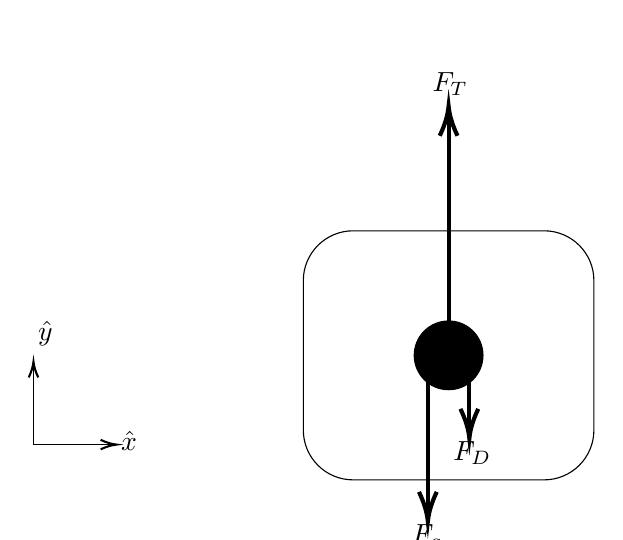
\begin{tikzpicture}[x=0.75pt,y=0.75pt,yscale=-1,xscale=1]
%uncomment if require: \path (0,308); %set diagram left start at 0, and has height of 308

%Rounded Rect [id:dp5842362308374554] 
\draw  [color={rgb, 255:red, 0; green, 0; blue, 0 }  ,draw opacity=1 ][fill={rgb, 255:red, 255; green, 255; blue, 255 }  ,fill opacity=1 ] (260,144) .. controls (260,130.75) and (270.75,120) .. (284,120) -- (376,120) .. controls (389.25,120) and (400,130.75) .. (400,144) -- (400,216) .. controls (400,229.25) and (389.25,240) .. (376,240) -- (284,240) .. controls (270.75,240) and (260,229.25) .. (260,216) -- cycle ;
%Straight Lines [id:da22630541270037763] 
\draw [line width=1.5]    (330,180) -- (330,63) ;
\draw [shift={(330,60)}, rotate = 90] [color={rgb, 255:red, 0; green, 0; blue, 0 }  ][line width=1.5]    (14.21,-4.28) .. controls (9.04,-1.82) and (4.3,-0.39) .. (0,0) .. controls (4.3,0.39) and (9.04,1.82) .. (14.21,4.28)   ;
%Straight Lines [id:da4912651471508729] 
\draw [line width=1.5]    (340,180) -- (340,217) ;
\draw [shift={(340,220)}, rotate = 270] [color={rgb, 255:red, 0; green, 0; blue, 0 }  ][line width=1.5]    (14.21,-4.28) .. controls (9.04,-1.82) and (4.3,-0.39) .. (0,0) .. controls (4.3,0.39) and (9.04,1.82) .. (14.21,4.28)   ;
%Shape: Circle [id:dp11471774870022611] 
\draw  [fill={rgb, 255:red, 0; green, 0; blue, 0 }  ,fill opacity=1 ] (313.44,180) .. controls (313.44,170.85) and (320.85,163.44) .. (330,163.44) .. controls (339.15,163.44) and (346.56,170.85) .. (346.56,180) .. controls (346.56,189.15) and (339.15,196.56) .. (330,196.56) .. controls (320.85,196.56) and (313.44,189.15) .. (313.44,180) -- cycle ;
%Straight Lines [id:da07105152032768414] 
\draw    (130,223) -- (130,185) ;
\draw [shift={(130,183)}, rotate = 90] [color={rgb, 255:red, 0; green, 0; blue, 0 }  ][line width=0.75]    (7.65,-2.3) .. controls (4.86,-0.97) and (2.31,-0.21) .. (0,0) .. controls (2.31,0.21) and (4.86,0.98) .. (7.65,2.3)   ;
%Straight Lines [id:da477096952774564] 
\draw    (130,223) -- (168,223) ;
\draw [shift={(170,223)}, rotate = 180] [color={rgb, 255:red, 0; green, 0; blue, 0 }  ][line width=0.75]    (7.65,-2.3) .. controls (4.86,-0.97) and (2.31,-0.21) .. (0,0) .. controls (2.31,0.21) and (4.86,0.98) .. (7.65,2.3)   ;
%Straight Lines [id:da5415789935745218] 
\draw [line width=1.5]    (320,180) -- (320,257) ;
\draw [shift={(320,260)}, rotate = 270] [color={rgb, 255:red, 0; green, 0; blue, 0 }  ][line width=1.5]    (14.21,-4.28) .. controls (9.04,-1.82) and (4.3,-0.39) .. (0,0) .. controls (4.3,0.39) and (9.04,1.82) .. (14.21,4.28)   ;

% Text Node
\draw (331,220.4) node [anchor=north west][inner sep=0.75pt]    {$F_{D}$};
% Text Node
\draw (321,42.4) node [anchor=north west][inner sep=0.75pt]    {$F_{T}$};
% Text Node
\draw (171,215.4) node [anchor=north west][inner sep=0.75pt]    {$\hat{x}$};
% Text Node
\draw (131,162.4) node [anchor=north west][inner sep=0.75pt]    {$\hat{y}$};
% Text Node
\draw (311,260.4) node [anchor=north west][inner sep=0.75pt]    {$F_{g}$};


\end{tikzpicture}
    \caption{1-DoF Forces on a body}
    \label{Figure 1}
\end{figure}

In Figure \ref{Figure 1}, a total of three forces are shown, all of which act along the  direction. The colinearity of all these forces is what makes this a 1-\gls{dof} model. The three forces shown are the thrust force, the drag force, and the gravity force.

Following what you may do in an introductory physics class, we will describe each of these forces via their functional form. These are described in Table \ref{Force Equations 1 DoF}. 

\begin{table}
\centering
\caption{Functional Form of Force Equations}
\label{Force Equations 1 DoF}
\begin{tabular}{l | l}
Force & Functional Form \\
\hline
 $F_g$&  $-mg$\\
 $F_D$&  $-\frac{1}{2} \rho_{\infty} V^2_{\infty}SC_D$\\
 $F_T$&  $F_T\cdot[1-u(t-t_b)], t\le0$\\

\end{tabular}

\end{table}
\newglossaryentry{freestream}
{
    name=freestream,
    first = {\textit{freestream}},
    description={A freestream quantity is one that is far away from the body, such that the influences of the body are negligible. For example, freestream velocity is the velocity that would be seen outside the influence of the body at the same conditions}
}

\newglossaryentry{ref area}
{
    name=reference area,
    first = \textit{reference area},
    description={An area that is used to define a characteristic area of an object in aerodynamics. This is used to normalize quantities such as lift and drag}
    }

    \newglossaryentry{drag coeff}
{
    name=drag coefficient,
    first = \textit{drag coefficient},
    description={A non dimensional parameter that describes the amount of drag acting on an object. This non-dimensionalized value is given by $\frac{F_D}{q_{\infty}S}$, where $q_{\infty}$ is the dynamic pressure, $\frac{1}{2}\rho_{\infty}V_{\infty}^2$}
    }
The notation here is important to understand. In future AAE classes at Purdue, this is likely the notation that you will see. Terms with the subscript $\infty$ denote \gls{freestream} quantities, those that are freely flowing far away from the body of interest. Also of note is the unit step function, which is a function which has value zero until reaching time $t_b$, where it thereafter equals one. The quantity  $\rho$ refers to the density of the fluid, and $S$ to the \gls{ref area}. The \gls{drag coeff} is $C_D$, a term which encapsulates the very complex nature of the fluid flow around an object. Calculating the value of  will be explored more deeply in later sections of this document. For now, we may assume a constant value.

It is helpful to think about these quantities as vectors, because we can add them together to achieve a resultant.\footnote{More formally, we define this as a linear space, where multiplicative and additive properties are preserved. This formal definition allows us to apply this to any arbitrarily number of dimensions. } In the 1-dimensional case this is quite trivial since all vectors along the $\hat{y}$ unit vector, but this will become increasingly important as we move to higher dimensions.
\subsection{Numerical Integration in the 1-DoF}\label{sec: Numerical Integration in the 1DoF}
Now we will move into something that you may have not seen before. Given all the forces, we normally apply Newton’s 2\textsuperscript{nd} Law, $\sum{\vec{F}}=m\vec{a}$ , to arrive at an expression for the acceleration as shown in \eqref{eq2}. Doing so might look something like this:
\begin{gather}
F_T \cdot [1-u(t-t_b)]-\frac{1}{2}\rho_{\infty}V_{\infty}^2SC_D-mg=m\vec{a}\label{eq1} \\
\vec{a}=\frac{F_T \cdot [1-u(t-t_b)]-\frac{1}{2}\rho_{\infty}V_{\infty}^2SC_D}{m}-g\label{eq2}
\end{gather}
 From here, we use integration to find the velocity and then position of the object with time. Formally, we might define this formally as:
 $$\vec{V}=\int{\vec{a}}{dt}$$
However, you may notice something strange with our equation. In our expression for acceleration, we need to know the velocity. However, we do not know the velocity without integrating the equation first. This puts us in a chicken v. egg situation, so we must take a different approach to the problem. \footnote{Sometimes systems like this can be solved with traditional ODE methods. However, most complex systems like our 6-\gls{dof} have no known analytical solutions. We will focus on numerical integration because it will be more useful in general. }

The way we resolve this is to make an approximation of the solution in a process called \textit{Numerical Integration. }Here, we will outline the simplest type of numerical integration, known as Euler’s Method. This section aims to show how to implement Euler’s method in code, and the mathematical reasoning will be given a more formal treatment in section 5. We will describe more complex numerical integration schemes and why you might want to use them, but it’s good to see the code for a simple case first.

Euler’s Method involves discretizing our time interval. You may remember the concept of a Riemann Sum from calculus, where you approximate an integral in discrete time steps. We will take a similar approach with Euler’s Method. Euler’s method is applicable to solving first order ordinary differential equations (ODE’s). However, in our problem, we have a second order differential equation, because $\vec{a}=\ddot{y}$.

To resolve this issue, we will make this one differential equation into a system of first order differential equations. In general, we can convert an nth-order ODE into a system of n first-order ODEs.

In this case, we define a variable, . Now, we can express equation \eqref{eq2} as a system of two differential equations:

\begin{gather}\label{system}
        \dot{v}=\frac{F_T \cdot [1-u(t-t_b)]-\frac{1}{2}\rho_{\infty}V_{\infty}^2SC_D}{m}-g\\
    \dot{y}=v
\end{gather}

Now, we will apply Euler’s method to solve the problem. We will use the following steps to do so, using equation \eqref{system}as our example:

1. Rewrite the system in Leibniz notation, where $\dot{x}=\frac{dx}{dt}$.

2. Perform separation of variables, to arrive at $dx=v\cdot dt$.

3. Discretize the equation by ‘converting’  $dx$ and $dt$ to $\Delta x$ and $\Delta t$.\footnote{Note that we are not ‘converting’ in the sense of an equality, since the equations are no longer equivalent when we convert a differential element into a discrete one. We are just making an approximation of the true solution. Luckily, numerical integration schemes can get us quite close to true solutions. }

4. Rewrite $\Delta x$ as $x_{new}-x_{old}$. We can rearrange the equation as $x_{new}=v\cdot \Delta t + x_{old}$

5. To start, we define an initial state. This initial state will be the first value of $x_{old}$. 

6. Iterate through values of $\Delta t$ until the desired time of simulation is achieved.

We follow the same process for the integration of acceleration to find the velocity. Of note, we will use the previous value of $v$ in the computation of the new acceleration. Note that a more formal definition of Euler’s method is given in section 5.1.

We also show this example in MATLAB Script \ref{Script 1} below. Note that $\frac{1}{2}\rho_{\infty}SC_D$ is called $k$ in the script for simplicity. This simplification assumes that $\rho_{\infty}$ and the $C_D$ are constant, which we will later see is a quite poor assumption but is okay for a first approximation.

\lstset{style=mystyle}

\lstinputlisting[language=Matlab, caption=1 DoF]{6DoF Explanation Scripts/OneDofEuler.m}\label{Script 1}

There are a few important things to note about the MATLAB implementation of the script. Firstly, the only force that is defined outside of the loop is gravity, because the magnitude and direction of this force is independent of the current state of the system. We contrast this with the drag force and the thrust, which must be calculated on every iteration through the algorithm to find an updated value for the force.

We also note the use of the Heaviside function. This is functionally identical to a unit step function, just a different notation.

\section{The 3-DoF Case}\label{sec: 3DoF Case}
\subsection{Vectors in the 3-DoF Case}
For particle dynamics, the most complex case is full 3D translational motion. Luckily, nothing very fundamental changes as compared to the 1-\gls{dof} case. The most important difference is the use of vector notation for compactness and clarity of mathematics and code. For position ($\vec{r}$), velocity ($\vec {v}$), and acceleration ($\vec{a}$), we represent them as tri-dimensional column vectors:

\begin{gather}
    \vec{r}=\begin{bmatrix}
        x_1\\
        x_2\\
        x_3
    \end{bmatrix},
    \vec{v}=\begin{bmatrix}
        \dot{x}_1\\
        \dot{x}_2\\
        \dot{x}_3\\
    \end{bmatrix},
        \vec{a}=\begin{bmatrix}
        \ddot{x}_1\\
        \ddot{x}_2\\
        \ddot{x}_3\\
    \end{bmatrix}
\end{gather}
This is done not only for the sake of compactness, but also to facilitate the use of matrix operations for translation between reference frames. This concept is further explored in section 3. For this reason, expressing these elements in vectors will become crucial as we move forward. In MATLAB, we express a tri-dimensional column vector as:
\begin{lstlisting}[language=Matlab]
pos=[0;0;0];
\end{lstlisting}
Where each semicolon represents a new row of the vector. We define a row vector by using a comma instead of a semicolon: 
\begin{lstlisting}[language=Matlab]
pos=[0,0,0];
\end{lstlisting}
Often, it is useful to convert between a row and column vector in MATLAB because some functions will expect the input to be in a different format. We can do so with a transposition. In MATLAB, this looks like: 
\begin{lstlisting}
pos=[0,0,0];
\end{lstlisting}
\subsection{Vector directions in the 3-DoF}\label{sec: vector directions in the 3DoF}
We present below a modified version of the 1-\gls{dof} below in full 3D in Figure \ref{fig:3 DoF Forces}.

\tikzset{every picture/.style={line width=0.75pt}} %set default line width to 0.75pt       

\begin{figure}[ht]
    \centering
    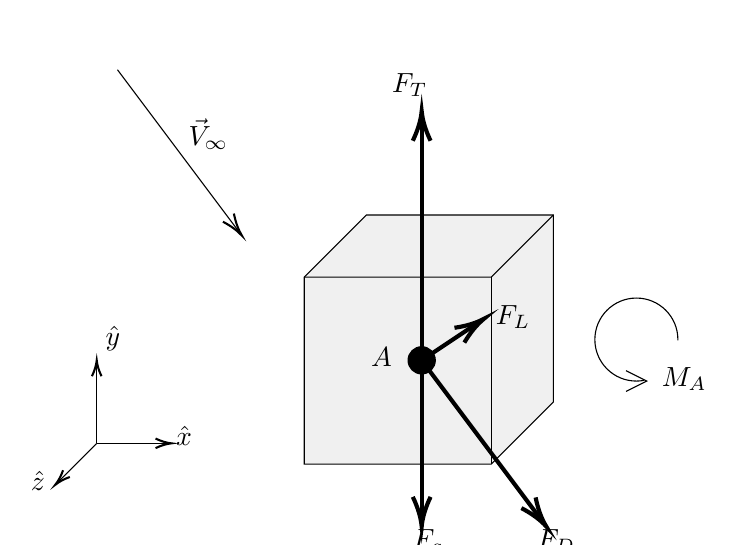
\begin{tikzpicture}[x=0.75pt,y=0.75pt,yscale=-1,xscale=1]
%uncomment if require: \path (0,308); %set diagram left start at 0, and has height of 308

%Shape: Cube [id:dp15885218660825062] 
\draw  [fill={rgb, 255:red, 155; green, 155; blue, 155 }  ,fill opacity=0.15 ] (260,129.92) -- (289.92,100) -- (380,100) -- (380,190.08) -- (350.08,220) -- (260,220) -- cycle ; \draw   (380,100) -- (350.08,129.92) -- (260,129.92) ; \draw   (350.08,129.92) -- (350.08,220) ;
%Straight Lines [id:da7537274804871096] 
\draw    (160,210) -- (160,172) ;
\draw [shift={(160,170)}, rotate = 90] [color={rgb, 255:red, 0; green, 0; blue, 0 }  ][line width=0.75]    (7.65,-2.3) .. controls (4.86,-0.97) and (2.31,-0.21) .. (0,0) .. controls (2.31,0.21) and (4.86,0.98) .. (7.65,2.3)   ;
%Straight Lines [id:da28051238395124845] 
\draw    (160,210) -- (194,210) ;
\draw [shift={(196,210)}, rotate = 180] [color={rgb, 255:red, 0; green, 0; blue, 0 }  ][line width=0.75]    (7.65,-2.3) .. controls (4.86,-0.97) and (2.31,-0.21) .. (0,0) .. controls (2.31,0.21) and (4.86,0.98) .. (7.65,2.3)   ;
%Straight Lines [id:da0491508391303197] 
\draw    (160,210) -- (141.41,228.59) ;
\draw [shift={(140,230)}, rotate = 315] [color={rgb, 255:red, 0; green, 0; blue, 0 }  ][line width=0.75]    (7.65,-2.3) .. controls (4.86,-0.97) and (2.31,-0.21) .. (0,0) .. controls (2.31,0.21) and (4.86,0.98) .. (7.65,2.3)   ;
%Straight Lines [id:da4424478744689285] 
\draw    (170,30) -- (228.8,108.4) ;
\draw [shift={(230,110)}, rotate = 233.13] [color={rgb, 255:red, 0; green, 0; blue, 0 }  ][line width=0.75]    (10.93,-3.29) .. controls (6.95,-1.4) and (3.31,-0.3) .. (0,0) .. controls (3.31,0.3) and (6.95,1.4) .. (10.93,3.29)   ;
%Straight Lines [id:da9341165159771404] 
\draw [line width=1.5]    (316.56,170) -- (316.56,247) ;
\draw [shift={(316.56,250)}, rotate = 270] [color={rgb, 255:red, 0; green, 0; blue, 0 }  ][line width=1.5]    (14.21,-4.28) .. controls (9.04,-1.82) and (4.3,-0.39) .. (0,0) .. controls (4.3,0.39) and (9.04,1.82) .. (14.21,4.28)   ;
%Straight Lines [id:da4700324062294746] 
\draw [line width=1.5]    (316.56,170) -- (374.76,247.6) ;
\draw [shift={(376.56,250)}, rotate = 233.13] [color={rgb, 255:red, 0; green, 0; blue, 0 }  ][line width=1.5]    (14.21,-4.28) .. controls (9.04,-1.82) and (4.3,-0.39) .. (0,0) .. controls (4.3,0.39) and (9.04,1.82) .. (14.21,4.28)   ;
%Straight Lines [id:da6206056974950449] 
\draw [line width=1.5]    (316.56,170) -- (316.56,53) ;
\draw [shift={(316.56,50)}, rotate = 90] [color={rgb, 255:red, 0; green, 0; blue, 0 }  ][line width=1.5]    (14.21,-4.28) .. controls (9.04,-1.82) and (4.3,-0.39) .. (0,0) .. controls (4.3,0.39) and (9.04,1.82) .. (14.21,4.28)   ;
%Shape: Circle [id:dp9278618893074794] 
\draw  [fill={rgb, 255:red, 0; green, 0; blue, 0 }  ,fill opacity=1 ] (310,170) .. controls (310,166.38) and (312.94,163.44) .. (316.56,163.44) .. controls (320.19,163.44) and (323.13,166.38) .. (323.13,170) .. controls (323.13,173.62) and (320.19,176.56) .. (316.56,176.56) .. controls (312.94,176.56) and (310,173.62) .. (310,170) -- cycle ;
%Straight Lines [id:da05847350311292765] 
\draw [line width=1.5]    (316.56,170) -- (344.07,151.66) ;
\draw [shift={(346.56,150)}, rotate = 146.31] [color={rgb, 255:red, 0; green, 0; blue, 0 }  ][line width=1.5]    (14.21,-4.28) .. controls (9.04,-1.82) and (4.3,-0.39) .. (0,0) .. controls (4.3,0.39) and (9.04,1.82) .. (14.21,4.28)   ;
%Shape: Arc [id:dp5580370574812169] 
\draw  [draw opacity=0] (423.67,179.66) .. controls (422.48,179.88) and (421.25,180) .. (420,180) .. controls (408.95,180) and (400,171.05) .. (400,160) .. controls (400,148.95) and (408.95,140) .. (420,140) .. controls (431.05,140) and (440,148.95) .. (440,160) .. controls (440,160.15) and (440,160.29) .. (440,160.44) -- (420,160) -- cycle ; \draw   (423.67,179.66) .. controls (422.48,179.88) and (421.25,180) .. (420,180) .. controls (408.95,180) and (400,171.05) .. (400,160) .. controls (400,148.95) and (408.95,140) .. (420,140) .. controls (431.05,140) and (440,148.95) .. (440,160) .. controls (440,160.15) and (440,160.29) .. (440,160.44) ;  
\draw   (415,175) -- (425,180) -- (415,185) ;

% Text Node
\draw (197,200.4) node [anchor=north west][inner sep=0.75pt]    {$\hat{x}$};
% Text Node
\draw (163,152.4) node [anchor=north west][inner sep=0.75pt]    {$\hat{y}$};
% Text Node
\draw (127,222.4) node [anchor=north west][inner sep=0.75pt]    {$\hat{z}$};
% Text Node
\draw (203,52.4) node [anchor=north west][inner sep=0.75pt]    {$\vec{V}_{\infty }$};
% Text Node
\draw (311,250.4) node [anchor=north west][inner sep=0.75pt]    {$F_{g}$};
% Text Node
\draw (371,250.4) node [anchor=north west][inner sep=0.75pt]    {$F_{D}$};
% Text Node
\draw (301,30.4) node [anchor=north west][inner sep=0.75pt]    {$F_{T}$};
% Text Node
\draw (351,142.4) node [anchor=north west][inner sep=0.75pt]    {$F_{L}$};
% Text Node
\draw (431,172.4) node [anchor=north west][inner sep=0.75pt]    {$M_{A}$};
% Text Node
\draw (291,162.4) node [anchor=north west][inner sep=0.75pt]    {$A$};


\end{tikzpicture}

    \caption{3-DoF Forces on a Body}
    \label{fig:3 DoF Forces}
\end{figure}
\newglossaryentry{angle of attack}
{
    name=angle of attack,
    first={\textit{angle of attack}},
    description={The angle of offset of the freestream velocity with the $\hat{X}$/$\hat{b}_1$, or longitudinal axis, of the vehicle. This is often denoted with the Greek letter $\alpha$}
}
As compared to 1-\gls{dof} case, we have three new quantities that are present. The first of these is $\vec{V}_{\infty}$, the freestream airflow vector, being shown on the diagram.\footnote{\gls{freestream} velocity  is drawn in the direction of incoming air by convention. However, for calculations, we will use the convention that  is the direction of the velocity of the vehicle (opposite sign to drawing).} This is represented diagrammatically because it no longer must be along the $\hat{y}$ direction. When we have an angle between the nose (the direction through which the thrust force points in Figure 2) and the \gls{freestream} velocity, we refer to this as an \gls{angle of attack}. This \gls{angle of attack} is often denoted with the letter $\alpha$. We will discuss \gls{angle of attack} and its effects more in section 4. For now, we simply need to understand how to calculate  given the vector through the nose and the \gls{freestream} velocity vector.

To do this, we use the fact that the dot product is related to the cosine of the angle between the vectors. Denoting the vector through the nose of the rocket , we can find the \gls{angle of attack} as:
\begin{equation}\label{eq:alpha}
    \alpha=cos^{-1}\left(\frac{\hat{X}\cdot \vec{V}_{\infty}}{||\hat{X}||\ ||\vec{V}_{\infty}||}\right)
\end{equation}

The next new quantity is $F_L$, the force of lift. The force of lift is always perpendicular in direction to $\vec{V}_{\infty}$. Knowing this, we can find the direction of the force of lift as:
\begin{equation}\label{eq:Lift}
    \hat{L}=\frac{(\hat{V}_{\infty} \times \hat{X}) \times \hat{V}_{\infty}}{||(\hat{V}_{\infty} \times \hat{X}) \times \hat{V}_{\infty}||}
\end{equation}
Here, the cross product is used because it generates a vector orthogonal to the two input vectors. This is exactly the property that we need when defining lift.

For the sake of completeness, we should also note that the force of drag lies opposite the direction of . This is much simpler to calculate, and looks like:
\begin{equation}\label{eq:drag}
\hat{D}=\frac{-\hat{V}_{\infty}}{||\hat{V}_{\infty}||}
\end{equation}

The last force directions to define are the direction of thrust and the direction of gravity. Luckily, these are easily defined because they point directly along basis vectors.\footnote{We assume here that there is no misalignment in the thrust vector and it is coincident with the  vector.} The force of gravity is defined with respect to the inertial reference frame and is defined in \eqref{eq:Fg}. The force of thrust is defined with respect to the vector pointing through the nose, $\hat{X}$, and is shown in \eqref{eq:Ft}:
\begin{equation}\label{eq:Fg}
    \vec{F}_g=-mg\cdot \hat{y}
\end{equation}
\begin{equation}\label{eq:Ft}
    \vec{F}_T=F_T\cdot \hat{X}
\end{equation}
\subsection{Moments}\label{sec:moments}
The last new quantity is the moment about point A, denoted $M_A$. For now, we will simply note that for an arbitrary selection of point A, we will have a rotational moment that is generated because the forces on the body do not necessarily act through point A, even if it is the center of mass (see section 4 for more details). In Figure\ref{fig:3 DoF Forces}, we have drawn all of the forces acting through a single point for simplicity, but this is not generally the case.

For our rocket modeling, it is generally assumed that gravity and thrust act about the center of gravity, and the aerodynamic forces about the center of pressure (more on this in 4.1.1).

We will show how to compute this moment if the location of the center of gravity and the center of pressure is known. To show this, we will briefly return the 2D case for illustration, but keep in mind that this concept is extensible in 3D. We show this in Figure \ref{fig:Moments}.

\begin{figure}
    \centering
    
\tikzset{every picture/.style={line width=0.75pt}} %set default line width to 0.75pt        

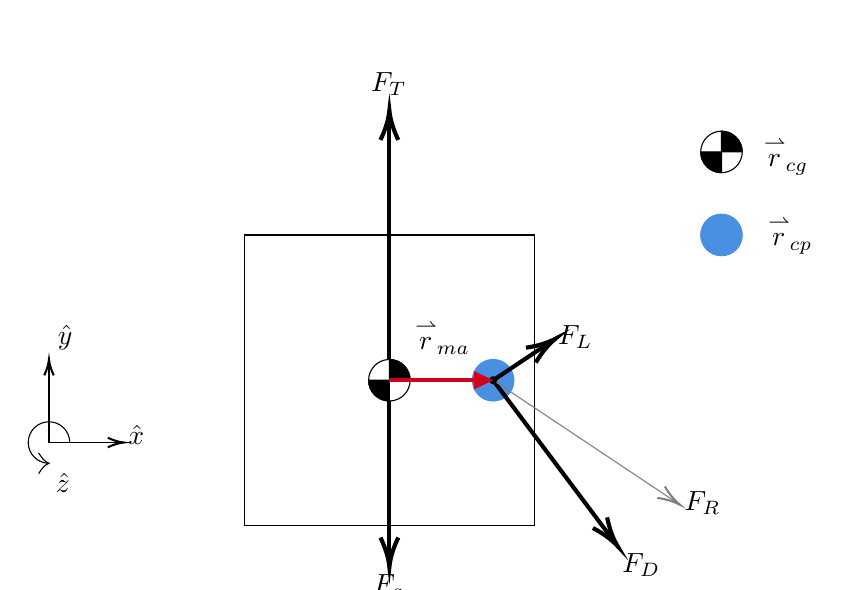
\begin{tikzpicture}[x=0.75pt,y=0.75pt,yscale=-1,xscale=1]
%uncomment if require: \path (0,300); %set diagram left start at 0, and has height of 300

%Shape: Rectangle [id:dp16059631350753278] 
\draw   (224,90) -- (364,90) -- (364,230) -- (224,230) -- cycle ;
%Shape: Circle [id:dp26152316559967836] 
\draw   (284,160) .. controls (284,154.48) and (288.48,150) .. (294,150) .. controls (299.52,150) and (304,154.48) .. (304,160) .. controls (304,165.52) and (299.52,170) .. (294,170) .. controls (288.48,170) and (284,165.52) .. (284,160) -- cycle ;
%Straight Lines [id:da4396178512453982] 
\draw [line width=1.5]    (294,150) -- (294,33) ;
\draw [shift={(294,30)}, rotate = 90] [color={rgb, 255:red, 0; green, 0; blue, 0 }  ][line width=1.5]    (14.21,-4.28) .. controls (9.04,-1.82) and (4.3,-0.39) .. (0,0) .. controls (4.3,0.39) and (9.04,1.82) .. (14.21,4.28)   ;
%Straight Lines [id:da6367078669315451] 
\draw [line width=1.5]    (294,170) -- (294,247) ;
\draw [shift={(294,250)}, rotate = 270] [color={rgb, 255:red, 0; green, 0; blue, 0 }  ][line width=1.5]    (14.21,-4.28) .. controls (9.04,-1.82) and (4.3,-0.39) .. (0,0) .. controls (4.3,0.39) and (9.04,1.82) .. (14.21,4.28)   ;
%Shape: Circle [id:dp9868324677149697] 
\draw  [color={rgb, 255:red, 74; green, 144; blue, 226 }  ,draw opacity=1 ][fill={rgb, 255:red, 74; green, 144; blue, 226 }  ,fill opacity=1 ] (334,160) .. controls (334,154.48) and (338.48,150) .. (344,150) .. controls (349.52,150) and (354,154.48) .. (354,160) .. controls (354,165.52) and (349.52,170) .. (344,170) .. controls (338.48,170) and (334,165.52) .. (334,160) -- cycle ;
%Straight Lines [id:da08375154983020605] 
\draw [line width=1.5]    (344,160) -- (371.5,141.66) ;
\draw [shift={(374,140)}, rotate = 146.31] [color={rgb, 255:red, 0; green, 0; blue, 0 }  ][line width=1.5]    (14.21,-4.28) .. controls (9.04,-1.82) and (4.3,-0.39) .. (0,0) .. controls (4.3,0.39) and (9.04,1.82) .. (14.21,4.28)   ;
%Straight Lines [id:da9997269035553926] 
\draw [line width=1.5]    (344,160) -- (402.2,237.6) ;
\draw [shift={(404,240)}, rotate = 233.13] [color={rgb, 255:red, 0; green, 0; blue, 0 }  ][line width=1.5]    (14.21,-4.28) .. controls (9.04,-1.82) and (4.3,-0.39) .. (0,0) .. controls (4.3,0.39) and (9.04,1.82) .. (14.21,4.28)   ;
%Straight Lines [id:da3915949331033487] 
\draw [color={rgb, 255:red, 128; green, 128; blue, 128 }  ,draw opacity=1 ]   (344,160) -- (432.34,218.89) ;
\draw [shift={(434,220)}, rotate = 213.69] [color={rgb, 255:red, 128; green, 128; blue, 128 }  ,draw opacity=1 ][line width=0.75]    (10.93,-3.29) .. controls (6.95,-1.4) and (3.31,-0.3) .. (0,0) .. controls (3.31,0.3) and (6.95,1.4) .. (10.93,3.29)   ;
%Shape: Circle [id:dp6233406826761347] 
\draw  [fill={rgb, 255:red, 0; green, 0; blue, 0 }  ,fill opacity=1 ] (342.33,160) .. controls (342.33,159.08) and (343.08,158.33) .. (344,158.33) .. controls (344.92,158.33) and (345.67,159.08) .. (345.67,160) .. controls (345.67,160.92) and (344.92,161.67) .. (344,161.67) .. controls (343.08,161.67) and (342.33,160.92) .. (342.33,160) -- cycle ;
%Shape: Pie [id:dp5263153723129019] 
\draw  [fill={rgb, 255:red, 0; green, 0; blue, 0 }  ,fill opacity=1 ] (294,150) .. controls (294,150) and (294,150) .. (294,150) .. controls (299.52,150) and (304,154.48) .. (304,160) -- (294,160) -- cycle ;
%Shape: Pie [id:dp03519524739615432] 
\draw  [fill={rgb, 255:red, 0; green, 0; blue, 0 }  ,fill opacity=1 ] (294,170) .. controls (294,170) and (294,170) .. (294,170) .. controls (294,170) and (294,170) .. (294,170) .. controls (288.48,170) and (284,165.52) .. (284,160) -- (294,160) -- cycle ;
%Straight Lines [id:da5638933773253405] 
\draw [color={rgb, 255:red, 208; green, 2; blue, 27 }  ,draw opacity=1 ][line width=1.5]    (294,160) -- (340,160) ;
\draw [shift={(344,160)}, rotate = 180] [fill={rgb, 255:red, 208; green, 2; blue, 27 }  ,fill opacity=1 ][line width=0.08]  [draw opacity=0] (9.29,-4.46) -- (0,0) -- (9.29,4.46) -- cycle    ;
%Shape: Circle [id:dp854204209250383] 
\draw   (444,50) .. controls (444,44.48) and (448.48,40) .. (454,40) .. controls (459.52,40) and (464,44.48) .. (464,50) .. controls (464,55.52) and (459.52,60) .. (454,60) .. controls (448.48,60) and (444,55.52) .. (444,50) -- cycle ;
%Shape: Pie [id:dp5370740069872785] 
\draw  [fill={rgb, 255:red, 0; green, 0; blue, 0 }  ,fill opacity=1 ] (454,60) .. controls (454,60) and (454,60) .. (454,60) .. controls (454,60) and (454,60) .. (454,60) .. controls (448.48,60) and (444,55.52) .. (444,50) -- (454,50) -- cycle ;
%Shape: Pie [id:dp7640770799900009] 
\draw  [fill={rgb, 255:red, 0; green, 0; blue, 0 }  ,fill opacity=1 ] (454,40) .. controls (454,40) and (454,40) .. (454,40) .. controls (459.52,40) and (464,44.48) .. (464,50) -- (454,50) -- cycle ;
%Shape: Circle [id:dp281241699306923] 
\draw  [color={rgb, 255:red, 74; green, 144; blue, 226 }  ,draw opacity=1 ][fill={rgb, 255:red, 74; green, 144; blue, 226 }  ,fill opacity=1 ] (444,90) .. controls (444,84.48) and (448.48,80) .. (454,80) .. controls (459.52,80) and (464,84.48) .. (464,90) .. controls (464,95.52) and (459.52,100) .. (454,100) .. controls (448.48,100) and (444,95.52) .. (444,90) -- cycle ;
%Straight Lines [id:da2704614420307284] 
\draw    (130,190) -- (130,152) ;
\draw [shift={(130,150)}, rotate = 90] [color={rgb, 255:red, 0; green, 0; blue, 0 }  ][line width=0.75]    (7.65,-2.3) .. controls (4.86,-0.97) and (2.31,-0.21) .. (0,0) .. controls (2.31,0.21) and (4.86,0.98) .. (7.65,2.3)   ;
%Straight Lines [id:da24091737468013485] 
\draw    (130,190) -- (164,190) ;
\draw [shift={(166,190)}, rotate = 180] [color={rgb, 255:red, 0; green, 0; blue, 0 }  ][line width=0.75]    (7.65,-2.3) .. controls (4.86,-0.97) and (2.31,-0.21) .. (0,0) .. controls (2.31,0.21) and (4.86,0.98) .. (7.65,2.3)   ;
%Shape: Arc [id:dp6249807559731687] 
\draw  [draw opacity=0] (130,200) .. controls (130,200) and (130,200) .. (130,200) .. controls (130,200) and (130,200) .. (130,200) .. controls (124.48,200) and (120,195.52) .. (120,190) .. controls (120,184.48) and (124.48,180) .. (130,180) .. controls (135.52,180) and (140,184.48) .. (140,190) -- (130,190) -- cycle ; \draw   (130,200) .. controls (130,200) and (130,200) .. (130,200) .. controls (130,200) and (130,200) .. (130,200) .. controls (124.48,200) and (120,195.52) .. (120,190) .. controls (120,184.48) and (124.48,180) .. (130,180) .. controls (135.52,180) and (140,184.48) .. (140,190) ;  
\draw   (125,195) .. controls (126.67,197.78) and (128.33,199.44) .. (130,200) .. controls (128.33,200.56) and (126.67,202.22) .. (125,205) ;

% Text Node
\draw (284,10.4) node [anchor=north west][inner sep=0.75pt]    {$F_{T}$};
% Text Node
\draw (285,252.4) node [anchor=north west][inner sep=0.75pt]    {$F_{g}$};
% Text Node
\draw (374,132.4) node [anchor=north west][inner sep=0.75pt]    {$F_{L}$};
% Text Node
\draw (405,242.4) node [anchor=north west][inner sep=0.75pt]    {$F_{D}$};
% Text Node
\draw (435,212.4) node [anchor=north west][inner sep=0.75pt]    {$F_{R}$};
% Text Node
\draw (305,130.4) node [anchor=north west][inner sep=0.75pt]    {$\stackrel {\rightharpoonup}{r}_{ma}$};
% Text Node
\draw (473,42.4) node [anchor=north west][inner sep=0.75pt]    {$\stackrel {\rightharpoonup}{r}_{cg}$};
% Text Node
\draw (475,80.4) node [anchor=north west][inner sep=0.75pt]    {$\stackrel {\rightharpoonup}{r}_{cp}$};
% Text Node
\draw (167,180.4) node [anchor=north west][inner sep=0.75pt]    {$\hat{x}$};
% Text Node
\draw (133,132.4) node [anchor=north west][inner sep=0.75pt]    {$\hat{y}$};
% Text Node
\draw (132,203.4) node [anchor=north west][inner sep=0.75pt]    {$\hat{z}$};


\end{tikzpicture}

    \caption{Moment Demonstration}
    \label{fig:Moments}
\end{figure}
In Figure \ref{fig:Moments} we include a few new symbols. All force magnitudes, however, are equivalent to what we show in Figure 2 (with the assumption that they lie in the x-y plane for this example). We denote the location of the center of gravity as $\vec{r}_{cg}$ and the location of the center of pressure as $\vec{r}_{cp}$. The difference between $\vec{r}_{cg}$ and $\vec{r}_{cp}$ is denoted as $\vec{r}_{ma}$. We refer to this as the moment arm of the aerodynamic forces. It should be noted that all of locations are tridimensional vectors. 

We also define a new vector, $F_R$, the resultant aerodynamic vector, which is the vector sum of $F_D$ and $F_L$. Because free rotations occur about the center of mass, it is most helpful to calculate our final moment from this location. To do so, we use the moment equation:
$$M=\vec{r}\times \vec{F}_R$$
\newacronym{rhr}{RHR}{right hand rule}
We note that the direction of this moment is in the $-\hat{z}$ direction from the \gls{rhr}. If we assume that our forces are planar, this moment will generate a rotation about a single axis. This effectively makes our model into a 4-\gls{dof}.

One thing to note is that some quantities are more easily defined with respect to vectors that are defined with respect to the vehicle (which we will call the \textit{body frame}), such as the vector $\hat{X}$. As seen in Equation \eqref{eq:alpha} and \eqref{eq:Lift}, we often want to use these vectors in the body frame for computation. As such, we will need a method in which we can convert between the body and inertial frames. This conversion between frames is explored in section \ref{sec:Frame of Reference}. We should also note that our moments will be in this body frame as well, which turns out to be especially useful in Section \ref{Euler Rotation Equations}.

The last thing that we note in this section is that our forces are moments are coupled. This means that the aerodynamic forces are a function of the orientation of the vehicle, so the moments and forces must be solved as a system.
\subsection{State Vector}
As a last note for this section, we will briefly discuss the concept of a \gls{state vector}. The \gls{state vector} is a column vector that contains information on the current state of our system. In the example of our 4-\gls{dof}, we will include the position, velocity, rotation, and rotation rate of the system in the \gls{state vector}. This would look like\footnote{The order of the state vector does not particularly matter, so long as we are consistent with the location of the elements. Typically, it is common to write all vectors first and then their derivatives, but there is no hard rule.}:
$$\vec{X}=\begin{bmatrix}
    x\\y\\z\\\theta\\\dot{x}\\\dot{y}\\\dot{z}\\\dot{\theta}
\end{bmatrix}$$
It is also useful to define the derivative of our \gls{state vector}, which would just be the derivative of each of its elements. This is expressed as
$$\dot{\textbf{X}}=\begin{bmatrix}
    \dot{x}\\\dot{y}\\\dot{z}\\\dot{\theta}\\\ddot{x}\\\ddot{y}\\\ddot{z}\\\ddot{\theta}
\end{bmatrix}$$
For the sake of compactness, these vectors are generally not written in their full form. In this text, we will often refer to a \gls{state vector} as just $\vec{X}$. Note that we also use the vector $\hat{X}$ to denote a unit vector in the body frame, so the difference in the hat becomes an important distinction here.
\section{Euler Rotation Equations}\label{Euler Rotation Equations}
\newglossaryentry{rigid body}
{
    name=rigid body,
    first=\textit{rigid body},
    description={A rigid body is a system of particles whose positions with respect to each other is fixed. Rigid body dynamics are the basis of our analysis of rotational dynamics}
}

\newglossaryentry{moment of inertia}
{
    name=moment of inertia,
    first={\textit{moment of inertia}},
    description={A measure of its resistance to rotational acceleration. It is in essence, the rotational analogue of mass. Often denoted with the letter $I$}
}

In Section \ref{sec:moments} we have explored the moments that are created when a force acts at a point that is not through the center of mass. Here, we will make the jump from particle dynamics into \gls{rigid body} dynamics.

In analogy to Newton's 2nd Law of motion, there is an equally important relationship for rotational dynamics. This equation is known as Euler's 2nd Law:
\begin{equation}\label{eq:Euler 2nd Law}
    \vec{M}^o=^{i}\frac{d\vec{H}^o}{dt}
\end{equation}
This equation reads as 'The moment about point $O$ is the inertial time derivative of the angular momentum, H, about point $O$'. The superscript $i$ refers to the fact that this derivative must be taken in the inertial frame.

We also have the relationship between angular momentum, $H$, and the \gls{moment of inertia}, $I$, for an rigid body that you have likely seen in physics classes:
\begin{equation}\label{eq:Iw}
    {}^i\vec{H}={}^iI\vec{\omega}
\end{equation}
You will notice that our moment of inertia here is defined with respect to the inertial frame. As a result, when our body changes orientation, the moment of inertia may also change!

Often however, it is more helpful to define this moment of inertia in terms of our body frame. We will go through this derivation of the moment of inertia below.
\subsection{Moment of Inertia and Inertia Tensor}\label{moment of inertia}
The moment of inertia of a body is a measure of its resistance to rotational acceleration. It is in essence, the rotational analogue of mass (mass is a measure of resistance to linear acceleration, by the same line of reasoning).

Since we need the moment of inertia to describe our relationship for angular momentum in \eqref{eq:Iw}, it is useful for us to see its derivation here.

We can start by showing that the mass of a region can be found by integrating the density over it's volume. Mathematically, we show this as:
$$\iiint\limits_V{\rho}{dV}$$
Similarly, we know that the moment of inertia of a particle is $mr^2$, which is it's mass multiplied with the length of the moment arm, $r$, squared. This is often referred to as the 'second moment' of mass. By integrating this second moment, we have:
$$\iiint\limits_V{\rho}{r^2}{dV}$$
It is useful to define the moment of inertia along each direction, though. We can rewrite $r$ in terms of $x$, $y$, and $z$ for each of the component directions:
\begin{gather}
    I_{xx}=\iiint\limits_V{\rho}{\left(y^2+z^2\right)}{dV}\\
    I_{yy}=\iiint\limits_V{\rho}{\left(x^2+z^2\right)}{dV}\\
    I_{zz}=\iiint\limits_V{\rho}{\left(x^2+y^2\right)}{dV}
\end{gather}
For our rocket, we will find that these are the only quantities that we need to define. However, in general, we also have three more quantities, which are called the product of inertia. This is defined by the product of two of our elements, such as $xy$. This will have the same dimensions as the quantity $r^2$, so it can be applied in a similar way to the moment of inertia. The product of inertia is defined as follows:
\begin{gather}
    I_{xy}=I_{yx}\iiint\limits_V{-xy\rho}{dV}\\
    I_{xz}=I_{zx}\iiint\limits_V{-xz\rho}{dV}\\
    I_{yz}=I_{zy}\iiint\limits_V{-yz\rho}{dV}
\end{gather}
For our rocket, because of the symmetry about the $\hat{X}$ axis, these quantities go to zero. However, for future implementations that may include fuel slosh and asymmetries, the products of inertia may be non-zero!
\newglossaryentry{inertia tensor}
{
    name={inertia tensor},
    first=\textit{inertia tensor},
    description={A matrix that describes the moment of inertia along each of the axes of a body. This matrix, often denoted $I$, transforms the angular velocity, $\omega$ into an angular momentum, $H$}
}
We express our \gls{inertia tensor}, denoted $I$, as the $3\times3$ matrix which contains the moments and products of inertia.
$$I=\begin{bmatrix}
    I_{xx}&I_{xy}&I_{xz}\\
    I_{yx}&I_{yy}&I_{yz}\\
    I_{zx}&I_{zy}&I_{zz}
\end{bmatrix}$$
For our rocket, we get the simplification that:
$$I=\begin{bmatrix}
    I_{xx}&0&0\\
    0&I_{yy}&0\\
    0&0&I_{zz}
\end{bmatrix}$$
\newglossaryentry{principle axes}
{
    name={principle axes},
    first=\textit{principle axes},
    description={The axes defined such that the products of inertia for a body are zero. These axes are the values that solve the eigenvalue problem $I\vec{\omega}=I^*\vec{\omega}$}
}
\newacronym{pmoi}{PMOI}{principle moment of inertia}
In fact, we can always find axes such that the products of inertia are zero. These are called the \gls{principle axes} and are important in other applications, such as structures \cite{baker_statics_2020}. For our rocket, it just happens that these \gls{principle axes} are the ones we have chosen to define as our body frame. The moment of inertia along these principle axes are solutions to the eigenvalue problem $I\vec{\omega}=I^*\vec{\omega}$, where $I^*$ is a scalar. Essentially, we are finding a matrix $I$ such that the output is just a scalar multiple of the input, $\omega$. We can see that having this property will greatly simplify our results. This is another reason why we like to perform many calculations in the body frame.

Using the inertia tensor, a matrix form of \eqref{eq:Iw}  is written as:
\begin{equation}\label{eq:IwVec}
    \vec{H}=I\vec{\omega}
\end{equation}
In the simplification using the principle axes, we often refer to the terms $I_{xx}$, $I_{yy}$, and $I_{zz}$ simply as $I_x$, $I_y$, and $I_z$. There are called the \glspl{pmoi}.
\subsection{Rotations in the Body Frame}\label{sec:rotations in the body frame}
Now that we have defined our inertia tensor in the body frame, it is useful to reexamine \eqref{eq:Euler 2nd Law} and \eqref{eq:Iw} to express them in terms of the body frame.
\newacronym{bke}{BKE}{Basic Kinematic Equation}
We can express equation \eqref{eq:Euler 2nd Law} in terms of the body frame using the \gls{bke}. We write this as:
\begin{equation}\label{eq:bke}
{}^i\frac{dH^o}{dt}={}^b\frac{dH^o}{dt}+{}^e\vec{\omega}^b\times H^o
\end{equation}
In the case of principle axes, \eqref{eq:IwVec} can be simplified to yield:
$${}^iH^o=I_x\omega_x\hat{b}_1+I_y\omega_y\hat{b}_2+I_z\omega_z\hat{b}_3$$
Plugging this result into \eqref{eq:bke}, we get the following:
$${}^i\frac{dH^o}{dt}={}^b\frac{d}{dt}\left(I_x\omega_x\hat{b}_1+I_y\omega_y\hat{b}_2+I_z\omega_z\hat{b}_3\right)+{}^e\vec{\omega}^b\times \left(I_x\omega_x\hat{b}_1+I_y\omega_y\hat{b}_2+I_z\omega_z\hat{b}_3\right)$$
Where ${}^e\vec{\omega}^b$ is $\omega_x\hat{b}_1+\omega_y\hat{b}_2+\omega_z\hat{b}_3$. The algebraic manipulation and vector math here is left as an exercise for the reader. Collecting the final terms, our final expression is:
$${}^iH^o=\left[I_x\dot{\omega}_x+\left(I_z-I_y\right)\right]\hat{b}_1+\left[I_y\dot{\omega}_y+\left(I_x-I_z\right)\right]\hat{b}_2+\left[I_z\dot{\omega}_z+\left(I_y-I_x\right)\right]\hat{b}_3$$
Equating this with the moments in the body frame that were found in \ref{sec:moments} as ${}^bM^o=M_x\hat{b}_1+M_y\hat{b}_2+M_z\hat{b}_3$, we arrive at the final form of our equations for Euler rotations\footnote{Very observant readers may notice that this form of the equation is technically \textit{slightly} incorrect, since our center of rotation, $O$, will change throughout the flight as the center of mass changes position. Thus, we will have some small effects that are not accounted for in this equation. For our purposes, these are ignored for simplicity. However, a more general approach that implements this may be used in the future if slosh modelling is implemented.}:
\begin{gather}\label{eq: moment equations}
    M_x=I_x\dot{\omega}_x+\left(I_z-I_y\right)\omega_y\omega_z\\
    M_y=I_y\dot{\omega}_y+\left(I_x-I_z\right)\omega_z\omega_x\\
    M_z=I_z\dot{\omega}_z+\left(I_y-I_x\right)\omega_y\omega_x
\end{gather}
We can rearrange this to a form that is more useful for us (although somewhat less sightly), putting the unknown $\dot\omega$ (we also refer to this quantity as the angular acceleration, $\vec{\alpha}$) quantities alone:
\begin{gather}\label{eq: moment eq 2}
    \dot{\omega}_x=\frac{M_x-\left(I_z-I_y\right)\omega_y\omega_z}{I_x}\\
    \dot{\omega}_y=\frac{M_y-\left(I_x-I_z\right)\omega_z\omega_x}{I_y}\\
    \dot{\omega}_z=\frac{M_z-\left(I_y-I_x\right)\omega_y\omega_x}{I_z}
\end{gather}
These sets of equations are especially powerful because they allows us to numerically integrate the angular velocity. Our moments can be found using Newtonian dynamics and the \glspl{pmoi} are quantities that are easily found using the integrals described above in section \ref{moment of inertia}. We will use these angular velocity derivatives extensively in sections \ref{sec:DescribeEulerRates} and \ref{sec: quaternion rates} to describe the time rate of change of the attitude of the rocket.

\chapter{Attitude Dynamics}\label{sec:attitude dynamics}
\begin{chapquote}{Lord Kelvin, 1892}
''Quaternions came from Hamilton after his really good work had been done; and, though beautifully ingenious, have been an unmixed evil to those who have touched them in any way, including Clerk Maxwell.''
\end{chapquote}
Attitude Dynamics is the math describing the orientation of a vehicle in space as the result of applied moments. Relying heavily on advanced mathematics, this concept is naturally more difficult to grasp. However, we hope that, here more than anywhere, our centralization of all basic necessary information to understand the topic eases the pain a little.\footnote{For further understanding, see section 8 for more provided materials. } In fact, don’t be afraid to reach out to either Hudson Reynolds (@Hudson Reynolds) or I (@Preston Wright) on Slack with questions! A final note on the section: many of the derivations closely follow both the process and notation of resources which will become available to you throughout your time here at Purdue AAE. These are the AAE340 class script by Professors Frueh and Longuski, and the AAE590 Attitude Dynamics and Control script by Professor Frueh. In addition, a handbook delving into all the nitty-gritty details of attitude determination and dynamics, following the derivations here and then some, is also available to aid in your understanding! % It's happening


% All editing for this section/relating to this section is now being done in a separate document

% THE QUATERNION SECTION IS BEING OVERHAULED IN THE NEW DOC DON'T REFERENCE ANYTHING HERE YET

\section{Frame of Reference}\label{sec:Frame of Reference}
Before attempting to describe the orientation of any random body in space, we must first discuss how and why this is possible. A frame of reference is an \textit{orthonormal} set within three-dimensional space. The orthonormal nature of the basis vectors that create every frame of reference allows for any other vector in three-dimensional space to be described as a linear combination of those three basis vectors (hence why we call it a basis for 3-space). This tool becomes incredibly useful within the study of Newtonian and Attitude Dynamics, as every \gls{state vector} can be broken down into three set “scalar” directions. Naturally, the question arises of how we determine which set directions to utilize, and so we will be discussing a few frames of reference critical to the creation of a 6-\gls{dof} and Aerospace engineering as a whole.
\subsection{The Inertial Frame}
The first and most important frame of reference is the \textit{inertial frame}. Typically denoted by $e$ or $i$ (we avoid $i$ in this case because of our heavy use of complex numbers), or in our case $(\hat{x},\hat{y},\hat{z})$, this motionless frame is the one that allows for the use of Newton’s second law in the first place, as the frame itself has “zero” translational and rotational movement.\footnote{An inertial frame can have some constant velocity and still be inertial. Of course, the earth has some velocity around the sun and with respect to the distant stars which we can approximate as constant for our time scales and thus ignore.} We say “zero” as this motion must be negligible in relation to the vehicle of interest. For example, this specific 6-\gls{dof} sets the inertial frame to be anchored within the Earth on the launch pad. And while we are well aware the Earth is moving and rotating through space at a non-zero rate, this motion is negligible relative to the motion of our vehicle which remains close to Earth within the atmosphere for a short period of time. Therefore, we can assume that the Earth acts appropriately as an inertial frame of reference, and Newton’s second law is valid for this frame. 

Returning to the specific example of a 6-\gls{dof}, the directions you set your basis vectors to point in are mostly left to the coder’s discretion. If your chosen directions retain the orthonormal nature of a frame of reference, as well as obeying \textit{the right-hand rule}, the choice is all yours. Within the example we are following, our inertial frame’s origin is anchored within the launch pad as previously stated. The first inertial basis vector points up perpendicular to the Earth’s surface, the second inertial basis vector points due East, while the third inertial basis vector follows the right-hand rule and points due North. An image for quick reference is provided below:

\begin{figure}[H]
\centering
\tikzset{every picture/.style={line width=0.75pt}} %set default line width to 0.75pt        
\begin{tikzpicture}[x=0.75pt,y=0.75pt,yscale=-1,xscale=1]
%uncomment if require: \path (0,356); %set diagram left start at 0, and has height of 356

%Shape: Axis 2D [id:dp4662897481397581] 
\draw  (244,205.18) -- (448.8,205.18)(264.48,52) -- (264.48,222.2) (441.8,200.18) -- (448.8,205.18) -- (441.8,210.18) (259.48,59) -- (264.48,52) -- (269.48,59)  ;
%Straight Lines [id:da8652713079639678] 
\draw    (278.8,190.2) -- (174.38,299.55) ;
\draw [shift={(173,301)}, rotate = 313.68] [color={rgb, 255:red, 0; green, 0; blue, 0 }  ][line width=0.75]    (10.93,-3.29) .. controls (6.95,-1.4) and (3.31,-0.3) .. (0,0) .. controls (3.31,0.3) and (6.95,1.4) .. (10.93,3.29)   ;
%Shape: Circle [id:dp9817397826908267] 
\draw  [fill={rgb, 255:red, 0; green, 0; blue, 0 }  ,fill opacity=1 ] (259.08,205.18) .. controls (259.08,202.2) and (261.5,199.78) .. (264.48,199.78) .. controls (267.46,199.78) and (269.88,202.2) .. (269.88,205.18) .. controls (269.88,208.16) and (267.46,210.58) .. (264.48,210.58) .. controls (261.5,210.58) and (259.08,208.16) .. (259.08,205.18) -- cycle ;

% Text Node
\draw (242,9) node [anchor=north west][inner sep=0.75pt]   [align=left] {Upward};
% Text Node
\draw (253,27.4) node [anchor=north west][inner sep=0.75pt]    {$\hat{x} ,\hat{e}_{1}$};
% Text Node
\draw (154,300.4) node [anchor=north west][inner sep=0.75pt]    {$\hat{y} ,\hat{e}_{2}$};
% Text Node
\draw (151,325) node [anchor=north west][inner sep=0.75pt]   [align=left] {East};
% Text Node
\draw (453,187.4) node [anchor=north west][inner sep=0.75pt]    {$\hat{z} ,\hat{e}_{3}$};
% Text Node
\draw (448,211) node [anchor=north west][inner sep=0.75pt]   [align=left] {North};
% Text Node
\draw (271.89,208.15) node [anchor=north west][inner sep=0.75pt]  [rotate=-0.04] [align=left] {Launchpad};


\end{tikzpicture}
    \caption{Inertial Frame Convention}
    \label{fig:InertialFrame}
\end{figure}

\subsection{The Body Frame}
The second most important frame of reference is the \textit{body frame}. Typically denoted by $b$, or in our case $(\hat{X},\hat{Y},\hat{Z})$, this frame of reference is always anchored at some point in the vehicle and allows us to describe the \gls{state vector} in relation to the vehicle itself. This frame is moving and rotating with respect to the inertial frame. For every body frame you create – from a frame for the entire vehicle to a frame for a small electronic part – you want simplicity. This means that in aerospace, it is necessary for a general body frame to have a basis vector pointing along the longitudinal axis of the vehicle, as well as one out a wing. In addition, it means at a zero angle of rotation, every basis vector of the body frame is parallel to the corresponding basis vector in the inertial frame. This is imperative to rotational dynamics, as the offset of each basis vector in the body frame will correspond to the pitch, yaw, and roll of the vehicle. But more on that later.

\begin{figure}[H]
\centering
    
\includegraphics[width=\linewidth]{BodyFrame.png}
    \caption{Typical Body Frame Orientation}
    \label{fig:BodyFrameTypical}
\end{figure}

For our current model, the body frame of our 6-\gls{dof} has its origin in the nose of the vehicle. It has the first body basis vector, $\hat{X}$, pointing up along the longitudinal axis of the rocket following standard convention. The second basis vector, $\hat{Y}$, points right due East when on the launch pad, and the third, $\hat{Z}$, points due North on the launch pad. We use the cardinal directions of the launchpad as not only are there no conventional wings on the rocket, but it allows body frame to be defined parallel to the corresponding inertial frame basis vectors. Note that they won’t remain pointing in these directions as the rocket moves through space, and they may not even begin parallel to the inertial axis to begin with if the rocket launches from a tilt.

\begin{figure}[H]
\centering
\tikzset{every picture/.style={line width=0.75pt}} %set default line width to 0.75pt        

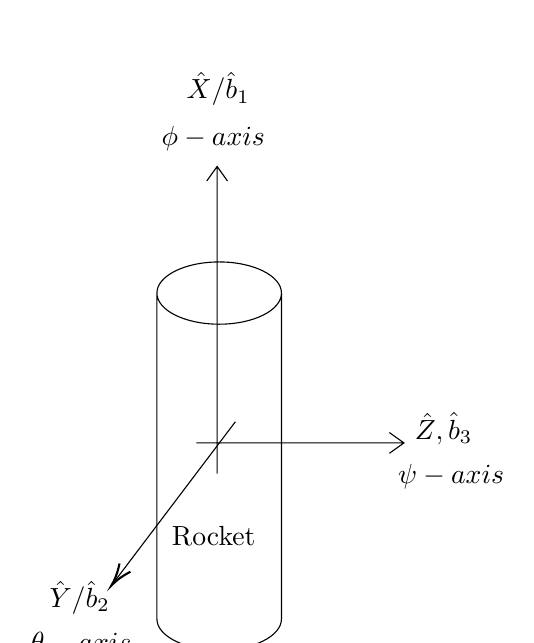
\begin{tikzpicture}[x=0.75pt,y=0.75pt,yscale=-1,xscale=1]
%uncomment if require: \path (0,408); %set diagram left start at 0, and has height of 408

%Shape: Can [id:dp7760621042562805] 
\draw   (351,111) -- (351,268) .. controls (351,276.28) and (337.57,283) .. (321,283) .. controls (304.43,283) and (291,276.28) .. (291,268) -- (291,111) .. controls (291,102.72) and (304.43,96) .. (321,96) .. controls (337.57,96) and (351,102.72) .. (351,111) .. controls (351,119.28) and (337.57,126) .. (321,126) .. controls (304.43,126) and (291,119.28) .. (291,111) ;
%Shape: Axis 2D [id:dp16563267347652144] 
\draw  (310,183.2) -- (410,183.2)(320,50) -- (320,198) (403,178.2) -- (410,183.2) -- (403,188.2) (315,57) -- (320,50) -- (325,57)  ;
%Straight Lines [id:da8489216589462083] 
\draw    (328.8,173) -- (270.21,250.41) ;
\draw [shift={(269,252)}, rotate = 307.12] [color={rgb, 255:red, 0; green, 0; blue, 0 }  ][line width=0.75]    (10.93,-3.29) .. controls (6.95,-1.4) and (3.31,-0.3) .. (0,0) .. controls (3.31,0.3) and (6.95,1.4) .. (10.93,3.29)   ;

% Text Node
\draw (304,3.4) node [anchor=north west][inner sep=0.75pt]    {$\hat{X} /\hat{b}_{1}$};
% Text Node
\draw (238,248.4) node [anchor=north west][inner sep=0.75pt]    {$\hat{Y} /\hat{b}_{2}$};
% Text Node
\draw (414,167.4) node [anchor=north west][inner sep=0.75pt]    {$\hat{Z} ,\hat{b}_{3}$};
% Text Node
\draw (297,222) node [anchor=north west][inner sep=0.75pt]   [align=left] {Rocket};
% Text Node
\draw (292,29.4) node [anchor=north west][inner sep=0.75pt]    {$\phi -axis$};
% Text Node
\draw (229,273.4) node [anchor=north west][inner sep=0.75pt]    {$\theta -axis$};
% Text Node
\draw (406,192.4) node [anchor=north west][inner sep=0.75pt]    {$\psi -axis$};

\end{tikzpicture}
    \caption{Body Frame Convention of our Rocket}
    \label{fig:BodyFrameRocket}
\end{figure}


%% Another Figure
\subsection{The Wind Frame}
The last and by far least important frame of reference is the \textit{wind frame.} This frame of reference, like the body frame, is always anchored at some point in the vehicle. Also like the body frame, it moves and rotates with the vehicle and allows for a new way of describing the \gls{state vector}. Unlike the body frame, the most important definition is not along the longitudinal axis of the vehicle. As indicated by its name, the necessary orientation of a basis vector points in the direction of the free stream velocity. Relating this to the body frame, this translates to an offset from the body frame by the \gls{angle of attack} and sideslip. This frame is often useful for aircraft, but we do not use it explicitly in our 6-\gls{dof}. The wind frame itself is in fact skipped over during wind calculations, as the \gls{angle of attack} and imparted forces/moments are calculated directly onto the body frame. So as this isn’t as useful as the other two reference frames, we won’t elaborate on this frame any further, and it won’t be shown as much in our example 6-\gls{dof}.

\section{2-D Rotations}\label{sec:2D Rotations}
Before moving into rotations in 3-dimensional space, let’s start simple. Say you have an arrow drawn on a piece of paper, and you twist the paper about the origin of that arrow through an angle $\theta$. While you could measure the new vector’s components directly to describe your new arrow, we want a more generalized way to find a new vector for any rotation. 
\subsection{Real Rotations}
\newglossaryentry{rhrRot}{
name={right hand rule (for rotations)},
first = \textit{right hand rule (for rotations)},
description = {This right hand rule helps determine the positive direction of rotation about an axis. Simpler than the previous right hand rule, you take your right hand and point your thumb in the direction of the axis you want to rotate about. Pretending to grasp the vector, the direction your fingers curl denotes the direction of positive rotation}
}
We will start the problem by defining our notation. We will utilize Cartesian coordinates with the positive $\hat{x}$ direction pointing to the right, $\hat{y}$ up, and $\hat{z}$ coming out of the page. Using this convention, a positive $\theta$ rotation is counterclockwise about the origin by use of the \gls{rhrRot}. We show an example of such a rotation in \ref{fig:2DRotation}:
%add glossary entry
\begin{figure}[H]
\centering

\tikzset{every picture/.style={line width=0.75pt}} %set default line width to 0.75pt        

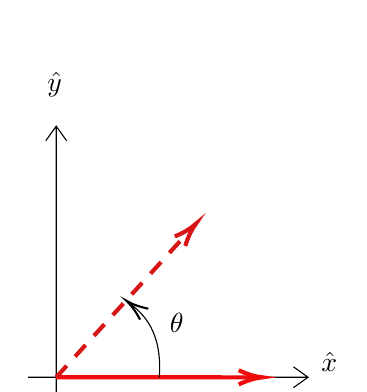
\begin{tikzpicture}[x=0.75pt,y=0.75pt,yscale=-1,xscale=1]
%uncomment if require: \path (0,300); %set diagram left start at 0, and has height of 300

%Shape: Axis 2D [id:dp2369017718792994] 
\draw  (274,169.56) -- (408.8,169.56)(287.48,48.6) -- (287.48,183) (401.8,164.56) -- (408.8,169.56) -- (401.8,174.56) (282.48,55.6) -- (287.48,48.6) -- (292.48,55.6)  ;
%Straight Lines [id:da6414021669220791] 
\draw [color={rgb, 255:red, 239; green, 11; blue, 11 }  ,draw opacity=1 ][line width=1.5]    (287.48,169.56) -- (383.8,169.6) ;
\draw [shift={(386.8,169.6)}, rotate = 180.02] [color={rgb, 255:red, 239; green, 11; blue, 11 }  ,draw opacity=1 ][line width=1.5]    (11.37,-3.42) .. controls (7.23,-1.45) and (3.44,-0.31) .. (0,0) .. controls (3.44,0.31) and (7.23,1.45) .. (11.37,3.42)   ;
%Straight Lines [id:da18731248462614536] 
\draw [color={rgb, 255:red, 215; green, 23; blue, 23 }  ,draw opacity=1 ][line width=1.5]  [dash pattern={on 5.63pt off 4.5pt}]  (287.48,169.56) -- (352.78,97.82) ;
\draw [shift={(354.8,95.6)}, rotate = 132.31] [color={rgb, 255:red, 215; green, 23; blue, 23 }  ,draw opacity=1 ][line width=1.5]    (11.37,-3.42) .. controls (7.23,-1.45) and (3.44,-0.31) .. (0,0) .. controls (3.44,0.31) and (7.23,1.45) .. (11.37,3.42)   ;
%Curve Lines [id:da22919468225468265] 
\draw    (337.14,169.58) .. controls (338.68,147.4) and (329.38,138.89) .. (322.7,133.77) ;
\draw [shift={(321.14,132.58)}, rotate = 37.01] [color={rgb, 255:red, 0; green, 0; blue, 0 }  ][line width=0.75]    (10.93,-3.29) .. controls (6.95,-1.4) and (3.31,-0.3) .. (0,0) .. controls (3.31,0.3) and (6.95,1.4) .. (10.93,3.29)   ;

% Text Node
\draw (341,137.4) node [anchor=north west][inner sep=0.75pt]    {$\theta $};
% Text Node
\draw (414,156.4) node [anchor=north west][inner sep=0.75pt]    {$\hat{x}$};
% Text Node
\draw (282,21.4) node [anchor=north west][inner sep=0.75pt]    {$\hat{y}$};


\end{tikzpicture}
    \caption{Example of 2-D Rotation}
    \label{fig:2DRotation}
\end{figure}
% do we want to use row vector when writing inline to make it cleaner?
Using this notation, we will express vectors as either column vectors of form:
$$\begin{bmatrix}
    x\\
    y
\end{bmatrix}$$
Or using the transpose of a row vector when we write them inline, as $\begin{bmatrix}
    x&y
\end{bmatrix}^T$.

In Figure \ref{fig:2DRotation}, our solid vector can be written as a unit vector $\begin{bmatrix}
    1&0
\end{bmatrix}^T$.
\newglossaryentry{linear}{
name={linear},
first = \textit{linear},
description = {An operation that preserves vector addition and scalar multiplication. Examples of linear operators include the derivative and integral. We also explore rotations as linear mappings}
}
With knowledge of linear algebra, we can see that the rotation of the vector is just some shearing of the original vector that preserves the vector length. These operations are \gls{linear}, so it is possible to find a matrix representation of this transformation.\footnote{We may also note that the property of preserving length means that our matrix must be \textit{unitary}. \textit{Unitary} matrices also preserve the inner product. Both of these are useful properties of these matrices. From these properties, it can also be shown that this matrix must be square.}

Mathematically, we want to find a square $2\times2$ matrix $R$ – called the rotation matrix – such that: $\vec{v}_2=R\vec{v}_1$
where $\vec{v}_1$ is our original vector, and $\vec{v}_2$ is our new, rotated vector. To derive our rotation matrix $R$, we will consider two similar vectors: our $\vec{v}_1$ mentioned above, as well as a new unit vector in the $\hat{y}$-direction 
$\begin{bmatrix}
    0&1
\end{bmatrix}^T$.
For each of our unit vectors, we will use 90- and 180-degree rotations, since we know what solution we should acquire for each. Those being 
$\begin{bmatrix}
    0&1
\end{bmatrix}^T$
and 
$\begin{bmatrix}
    -1&0
\end{bmatrix}^T$
respectively for our first unit vector. 
Using the initial equation given above paired with our first 90-degree rotation, we get
$$\begin{bmatrix}
    0\\1
\end{bmatrix}=R
\begin{bmatrix}
    1\\0
\end{bmatrix}$$
Based off our knowledge of trigonometry, we already know that some combination of sines and cosines will construct our matrix $R$. With our choice of the $\hat{x}$-direction unit vector, only the first column of $R$, $\begin{bmatrix}
    r_{11}&r_{21}
\end{bmatrix}^T$, will remain after matrix multiplication. This allows for the first column of $R$ to be solved as
$$\begin{bmatrix}
    0\\1
\end{bmatrix}=
\begin{bmatrix}
    r_{11}\\r_{21}
\end{bmatrix}
$$
And with a 90 degree rotation, $r_{21}$ can be determined to be $sin(\theta)$. Moving on to the second rotation, we use the equation 
$$\begin{bmatrix}
    -1\\0
\end{bmatrix}=R
\begin{bmatrix}
    1\\0
\end{bmatrix}$$
Repeating the above process, we get:
$$\begin{bmatrix}
    -1\\0
\end{bmatrix}=
\begin{bmatrix}
    r_{11}\\sin(\theta)
\end{bmatrix}$$
At a rotation of 180 degrees, $r_{11}$ must be $cos(\theta)$. We have now completed the first column of $R$: $\begin{bmatrix}
    cos(\theta)&sin(\theta)
\end{bmatrix}^T$. If we plot the rotated unit vector as a function of $\theta$ from [0, 360) degrees, we can see that we do indeed get the unit circle.
For the $\hat{y}$ unit vector we follow an identical process and derive the second column of $R$. This derivation will be left as an exercise to the reader due to the redundancy and simplicity of the process; however, we end up with $\begin{bmatrix}
    -sin(\theta)&cos(\theta)
\end{bmatrix}^T$ as our second column vector. Putting the two together, we have our completed rotation matrix:
\begin{equation}\label{eq:2DMatrix}
    R=
    \begin{bmatrix}
        cos(\theta)&-sin(\theta)\\sin(\theta)&cos(\theta)
    \end{bmatrix}
\end{equation}
The understanding of this derivation is helpful to the understanding of the derivation of the rotation matrix in 3-dimensional space, so we will be sure to keep this process handy!

\subsection{Imaginary Rotations}\label{sec:2DImaginary}
After deriving the matrix for rotations in regular 2-dimensional space, we can use this to describe the rotation of a vector in imaginary space. These results will serve as a basis for the motivation of quaternion rotations, which will be discussed later. 

To derive an expression for complex rotations, we will start with the famous Euler's Formula:
\begin{equation}
    e^{i\theta}=cos\theta+i\cdot sin\theta
\end{equation}
A succinct and intuitive explanation of Euler's Formula is given in two 3Blue1Brown videos, shown in sources \cite{3blue1brown_eipi_2019} and \cite{3blue1brown_how_2021}. Because these videos so expertly describe this topic, we choose not to do so here. As an exercise to the reader, you can try proving this statement yourself by considering the Taylor Series expansion of $e^{ix}$ and comparing it with the Taylor Series of $sin(x)$ and $cos(x)$.

So, since the magnitude of $e^{i\theta}$ is always 1, we can parameterize the length of our vector as its magnitude, $r$.

So, we now have a complex rotator which we can describe as:
\begin{gather}
    r=cos(\theta)+isin(\theta)\\
    \text{or}\\
    r=e^{i\theta}
\end{gather}
This way, any rotation $\theta$ here is an identical to a rotation of the same above, notation and all. We are simply replacing our x-axis with our real axis, and our y-axis with our imaginary axis. From this equality, we see that multiplication of a complex number corresponding to the appropriate real and imaginary components with the above complex rotator will result in an identical rotation to the same initial conditions in 2-dimensional space. To explicitly show this, we can express our imaginary rotation as matrix multiplication for the rotation of an imaginary number $\vec{v}=v_1+v_2i$:
$$\begin{bmatrix}
    v_1'\\v_2'
\end{bmatrix}=
\begin{bmatrix}
    cos(\theta)&-sin(\theta)\\sin(\theta)&cos(\theta)
\end{bmatrix}\begin{bmatrix}
    v_1\\v_2
\end{bmatrix}$$

One thing to note here is that we can express a rotation very cleanly and naturally with complex numbers and exponentials. When we discuss quaternions in Section \ref{sec:quaternions}, these complex numbers will become increasingly important to understand.
\section{Euler Angles}

\newglossaryentry{Euler angles}
{
    name=Euler angles,
    first = {\textit{Euler angles}},
    description={A group of three scalar values used to describe the orientation of a body in space}
}



\subsection{3-D Rotations}\label{sec:3DRotations}



\subsection{The Direction Cosine Matrix}\label{sec:TheDCM}


\subsection{Describing Angular Velocity with Euler Angles and Rates}

\newglossaryentry{Euler rates}
{
    name=Euler rates,
    first={\textit{Euler rates}},
    description={A way to describe rotational rates with orientation for 3-dimensional rotations, they are denoted by the dot of the corresponding Euler angle: ($\dot{\psi},\dot{\theta},\dot{\phi}$)}
}



\subsection{Describing Euler rates with Angular Velocities and Euler Angles}\label{sec:DescribeEulerRates}



\section{Quaternions}\label{sec:quaternions}
\newglossaryentry{quaternion}
{
    name=quaternion,
    first = {\textit{quaternion}},
    description={An extension of the complex numbers with elements $j$ and $k$ added. The common form is expressed $q_1+q_2i+q_3j+q_4k$ (our notation) or $q_1i+q_2j+q_3k+q_4$. The algebra of quaternions is generally denoted $\mathbb{H}$}
}
It was a gorgeous October day in Dublin, and William Hamilton was on a stroll with his wife on his way to the Royal Irish Academy. Having worked on hyper-imaginary numbers for some time, answers had been slowly forming in his head. As he crossed a cobblestone bridge above the Royal Canal, the answer of a necessary, fourth dimension for calculating triples struck him like a freight train. He hastily carved the fundamental formula for quaternion multiplication, $i^2+j^2+k^2=ijk=-1$, into the stones he was walking on. And so, \glspl{quaternion} were born.

\subsection{Quaternion Notation}


\newglossaryentry{versor}
{
    name=versor,
    first = {\textit{versor}},
    description={The normalization of a quaternion and the only way to encode rotations, it is equivalent to $\frac{\vec{q}}{||\vec{q}||}$. Fun note on the etymology of the word: it is derived from the Latin word ''versari'' which means ''to turn'' among other translations. With the suffix ''-or'', it becomes a noun, taking the meaning ''the turner''}
}

\subsection{Quaternion Mathematics}

\subsubsection{Addition}

\subsubsection{Scalar Multiplication}

\subsubsection{Quaternion Multiplication}

\subsubsection{Hamiltonian Product}

\subsubsection{Identity Quaternion}

\subsubsection{Conjugate of Quaternions}

\subsubsection{Inverse of Quaternions}





\subsection{Principal Axis Rotation Theorem}
\newglossaryentry{Euler axis}
{
    name=Euler axis,
    first = {\textit{Euler axis}},
    description={The axis about which a rotation of a body in space can be described by only a single rotation, denoted by $\vec{e}$}
}





\subsection{Compounding 2-Dimensional Rotations (Method I)}

\subsection{Relating Quaternions to Euler Angles (Method II)}

\subsection{Principle Axis Rotation Matrix (Method III)}\label{sec:PrincipleAxisRotationMatrix}

\newglossaryentry{skew-symmetric matrix}
{
    name=skew-symmetric matrix,
    first = {\textit{skew-symmetric matrix}},
    description={A matrix which obeys the property that every $a_{ij}=-a_{ji}$. This can be interpreted to mean every term across the diagonal is equal in magnitude, but opposite in sign. Sometimes called an anti-symmetric matrix or anti-metric matrix}
}



\subsection{Quaternion Rotation Matrix}



\subsection{Quaternion Rates}\label{sec: quaternion rates}





\section{Individual and Comprehensive Mathematical Proofs using MATLAB}\label{sec:MathematicalProofRotations}

In this section, we will use MATLAB to confirm proper derivations and prove the equality of multiple cases from the entirety of the previous chapter. As a whole, the section will be separated into four parts: 2-dimensional rotations, Euler angles, quaternions, and a comprehensive comparison of Euler angles and quaternions. The purpose of this section is not only to verify the theoretical mathematics highlighted throughout the sections above, but also to give insight into the use of MATLAB's built-in functions relating to Attitude Dynamics.



\section{3D Rotation Example: Dzhanibekov effect}\label{sec:Dzhan}

\newglossaryentry{dzhan}
{
    name={Dzhanibekov Effect},
    first=\textit{Dzhanibekov Effect},
    description={A phenomenon in which rotation about an intermediate axis results in rotation about another axis. This phenomenon occurs with any body where the three PMOIs are not equal. It is easily seen with a tennis racket or a cell phone},
    see={pmoi}
}
To help digest the complex nature of attitude dynamics, a full example is especially useful. One of the consequences of Euler's Equations described %eqref equation above
above is that rotation about an intermediate axis is unstable. This effect is known as the Intermediate Axis Theorem or the \gls{dzhan}.

This is a good phenomenon to describe 3D rotations because it requires us to put together lots of knowledge throughout this section. Because our object rotates about all three axes, we must parametrize our rotation with \glspl{quaternion} to avoid possible singularities in the solution.

Before we can describe our system dynamics, we need to establish our coordinate system for this problem.

\begin{figure}[ht]
    \centering


\tikzset{every picture/.style={line width=0.75pt}} %set default line width to 0.75pt        

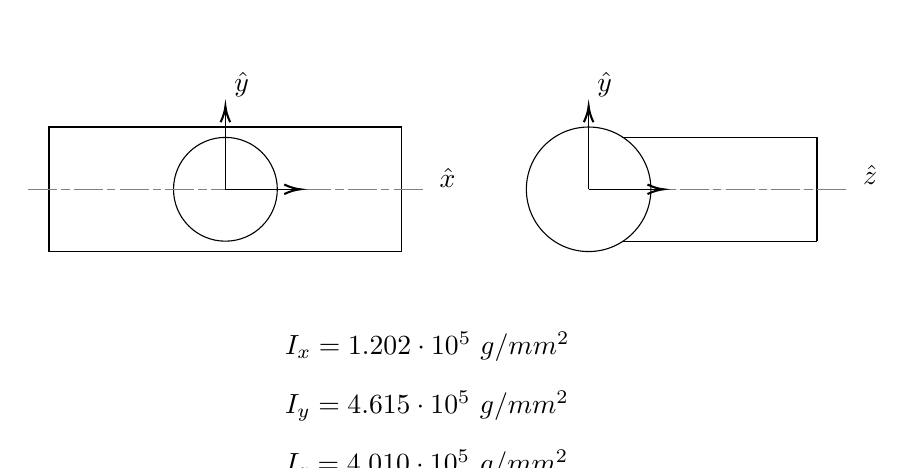
\begin{tikzpicture}[x=0.75pt,y=0.75pt,yscale=-1,xscale=1]
%uncomment if require: \path (0,300); %set diagram left start at 0, and has height of 300


%Shape: Circle [id:dp7493270463079389] 
\draw   (195,100) .. controls (195,86.19) and (206.19,75) .. (220,75) .. controls (233.81,75) and (245,86.19) .. (245,100) .. controls (245,113.81) and (233.81,125) .. (220,125) .. controls (206.19,125) and (195,113.81) .. (195,100) -- cycle ;
%Shape: Rectangle [id:dp8745965352536226] 
\draw   (135,70) -- (305,70) -- (305,130) -- (135,130) -- cycle ;
%Straight Lines [id:da5356768971699141] 
\draw [color={rgb, 255:red, 128; green, 128; blue, 128 }  ,draw opacity=1 ] [dash pattern={on 10.5pt off 1.5pt on 3pt off 1.5pt}]  (125,100) -- (315,100) ;
%Shape: Circle [id:dp11124327189723426] 
\draw   (365,100) .. controls (365,83.43) and (378.43,70) .. (395,70) .. controls (411.57,70) and (425,83.43) .. (425,100) .. controls (425,116.57) and (411.57,130) .. (395,130) .. controls (378.43,130) and (365,116.57) .. (365,100) -- cycle ;
%Straight Lines [id:da07234932776274916] 
\draw    (220,100) -- (220,62) ;
\draw [shift={(220,60)}, rotate = 90] [color={rgb, 255:red, 0; green, 0; blue, 0 }  ][line width=0.75]    (7.65,-2.3) .. controls (4.86,-0.97) and (2.31,-0.21) .. (0,0) .. controls (2.31,0.21) and (4.86,0.98) .. (7.65,2.3)   ;
%Straight Lines [id:da6659026149277345] 
\draw    (220,100) -- (254,100) ;
\draw [shift={(256,100)}, rotate = 180] [color={rgb, 255:red, 0; green, 0; blue, 0 }  ][line width=0.75]    (7.65,-2.3) .. controls (4.86,-0.97) and (2.31,-0.21) .. (0,0) .. controls (2.31,0.21) and (4.86,0.98) .. (7.65,2.3)   ;
%Straight Lines [id:da8158592711011072] 
\draw    (411,75) -- (505,75) ;
%Straight Lines [id:da1507348050424776] 
\draw    (411,125) -- (505,125) ;
%Straight Lines [id:da9455565481798273] 
\draw    (505,125) -- (505,75) ;
%Straight Lines [id:da5972499541109577] 
\draw [color={rgb, 255:red, 128; green, 128; blue, 128 }  ,draw opacity=1 ][fill={rgb, 255:red, 128; green, 128; blue, 128 }  ,fill opacity=1 ] [dash pattern={on 10.5pt off 1.5pt on 3pt off 1.5pt}]  (395,100) -- (520,100) ;
%Straight Lines [id:da4230804170313147] 
\draw    (395,100) -- (395,62) ;
\draw [shift={(395,60)}, rotate = 90] [color={rgb, 255:red, 0; green, 0; blue, 0 }  ][line width=0.75]    (7.65,-2.3) .. controls (4.86,-0.97) and (2.31,-0.21) .. (0,0) .. controls (2.31,0.21) and (4.86,0.98) .. (7.65,2.3)   ;
%Straight Lines [id:da58307827964758] 
\draw    (395,100) -- (429,100) ;
\draw [shift={(431,100)}, rotate = 180] [color={rgb, 255:red, 0; green, 0; blue, 0 }  ][line width=0.75]    (7.65,-2.3) .. controls (4.86,-0.97) and (2.31,-0.21) .. (0,0) .. controls (2.31,0.21) and (4.86,0.98) .. (7.65,2.3)   ;


% Text Node
\draw (322,88.4) node [anchor=north west][inner sep=0.75pt]    {$\hat{x}$};
% Text Node
\draw (223,42.4) node [anchor=north west][inner sep=0.75pt]    {$\hat{y}$};
% Text Node
\draw (398,42.4) node [anchor=north west][inner sep=0.75pt]    {$\hat{y}$};
% Text Node
\draw (526,87.4) node [anchor=north west][inner sep=0.75pt]    {$\hat{z}$};
% Text Node
\draw (247.5,167.4) node [anchor=north west][inner sep=0.75pt]    {$I_{x} =1.202\cdot 10^{5} \ g/mm^{2}$};
% Text Node
\draw (247.5,195.9) node [anchor=north west][inner sep=0.75pt]    {$I_{y} =4.615\cdot 10^{5} \ g/mm^{2}$};
% Text Node
\draw (247.5,224.4) node [anchor=north west][inner sep=0.75pt]    {$I_{z} =4.010\cdot 10^{5} \ g/mm^{2}$};


\end{tikzpicture}

    \caption{Non-Symmetric Body for Demonstrating Dzhanibekov Effect}
    \label{fig:Dzhan}
\end{figure}

\subsection{State Vector}
We'll start by describing our \gls{state vector} and initial conditions for this problem:

We define our original position is at the origin, giving us a position vector:
$$\vec{r}_0=\begin{bmatrix}
    0\\0\\0
\end{bmatrix}$$
We also define the initial velocity to be zero, giving a velocity vector:
$$\vec{v}_0=\begin{bmatrix}
    0\\0\\0
\end{bmatrix}$$
We also need an initial orientation. We can either directly initialize a \gls{quaternion} or write our initial orientation with \gls{Euler angles} and then convert to \glspl{quaternion}. Often, \gls{Euler angles} are more intuitive, so we will use these for our initialization. We can define an initial angle of all zeros, meaning that our body frame axes are initially coincident with the inertial frame. This gives \gls{Euler angles} of:
$$\begin{bmatrix}
    \phi\\\theta\\\psi
\end{bmatrix} =
\begin{bmatrix}
    0\\0\\0
\end{bmatrix}$$
Using the command "eul2quat" with a specification of "XYZ" for the frame, the initial \gls{quaternion} vector is given as:
$$\vec{q}_0=\begin{bmatrix}
    1\\0\\0\\0
\end{bmatrix}$$
Lastly, we need to describe the initial angular velocity. To properly demonstrate the effect, we need a small perturbation on our non-intermediate axes. We can write our omega vector as:
$$\vec{\omega}_0=\begin{bmatrix}
0.05\\0.05\\\pi
\end{bmatrix} rad/s$$

Putting all of the together, we arrive at our \gls{state vector}:
$$\vec{X}_0=\begin{bmatrix}
    \vec{r}_0\\\vec{v}_0\\\vec{\omega}_0\\\vec{q}_0
\end{bmatrix}$$
Which we can expand to the full form as a 13-element column vector:
$$\vec{X}_0=\begin{bmatrix}
    0\\0\\0\\0\\0\\0\\0.05\\0.05\\\pi\\1\\0\\0\\0
\end{bmatrix}$$
\subsection{Forces and Moments}
We can assume that we are operating in a 0-g environment (as this is where the effect is most prevalent) and that no body forces are acting on the object. We will also assume that air resistance in negligible and there are no losses. These assumptions mean that there are no forces that the acting on our body. Additionally, there are no moments on the body either. We have chosen this case for our example so that we can focus solely on the attitude dynamics.
\subsection{Attitude Dynamics}
Our attitude dynamics are fairly simple since there are no moments acting on the body. Our equations for the angular velocity rates in \eqref{eq: moment eq 2} reduce to:
\begin{gather}\label{eq: moment eq dzhan}
    \dot{\omega}_x=\frac{\left(I_y-I_z\right)\omega_y\omega_z}{I_x}\\
    \dot{\omega}_y=\frac{\left(I_z-I_x\right)\omega_z\omega_x}{I_y}\\
    \dot{\omega}_z=\frac{\left(I_x-I_y\right)\omega_y\omega_x}{I_z}
\end{gather}
To find our \gls{quaternion} rates, we simply use the same methods as in section \ref{sec: quaternion rates}. This gives us:
\begin{equation}
    \dot{\textbf{q}}=\frac{1}{2}\begin{bmatrix}
        0&-\omega_x&-\omega_y&-\omega_z\\
        \omega_x&0&\omega_z&-\omega_y\\
        \omega_y&-\omega_z&0&\omega_x\\
        \omega_z&\omega_y&-\omega_x&0
    \end{bmatrix}\vec{q}
\end{equation}
\subsection{Translating to Code}
With all of these defined, we can write the derivative of our \gls{state vector} as:
\begin{equation}
    \dot{\textbf{X}}=\begin{bmatrix}
        \vec{v}\\\vec{a}\\\vec{\alpha}\\\dot{\textbf{q}}
    \end{bmatrix}
\end{equation}
From here, we can implement this in "ode45". We show all of the code for this model in the appendix.

Our initialization of the \gls{state vector} and all of the basic setup in contained in the main file, shown in listing \ref{code:DzhanMain}. The code that gets the derivative of the \gls{state vector} is the function passed into ode45. This code is shown in listing \ref{code:DzhanInt}. There is additionally a file to display the rotation of the body in an animation, which is shown in listing \ref{code:DzhanRotVis}.

%% add listings.
\chapter{Aerodynamic Modeling}\label{sec: aerodynamics}
\begin{chapquote}{Werner Heisenberg}
''When I meet God, I am going to ask him two questions: Why relativity? And why turbulence? I really believe he will have an answer for the first.''
\end{chapquote}
In Section \ref{sec: 3DoF Case} we discussed the 4 fundamental forces on a vehicle and how we define their directions. In that section we did not define the magnitude of the aerodynamic forces, $F_L$ and $F_D$. The magnitude of these forces are quite difficult to calculate and require the most approximation to do correctly. The governing equation for calculating the magnitude of our aerodynamics is $\frac{1}{2}\rho_{\infty}V^2_{\infty}SC_X$, where $C_X$ is either $C_L$ or $C_D$.

% buckingham pi derivation of CD and CL - hugo

Despite the innocuous appearance of this equation, calculating the aerodynamics of our system is deceptively hard because the calculation of $C_X$ is very complicated. In fact, without real data, any calculation that we made of these values will just be an approximation.\footnote{Even with wind tunnel data, it is still likely that some approximations need to be made. Aerodynamics in general has no definite answers.} That being said, there are approaches we can take which will get us close enough to true values to prove useful.

\section{Aerodynamics Terminology}
Aerodynamics has a lot of terminology associated with it that is important to understand before we can approach modeling the aerodynamics of the system. We will mostly cover aerodynamics terminology for rockets, but the modeling done here should be transferable to aspects of aircraft systems as well.\footnote{The principles we describe are the same, but much of the modelling is simpler for rockets since they have axial symmetry in most cases. We will utilize these assumptions early on to simplify this section.}

While some of the theory here is not directly used in our 6-\gls{dof}, having an understanding of this will be greatly beneficial so we have chosen to include some background here. 
\subsection{Lift and Drag}\label{Lift and Drag}
We start this section by noting that lift and drag are just conventions that are commonly used to describe the aerodynamic force. It should be noted that both the lift and the drag arise from the same source - the air acting on the vehicle to create a force. It is simply convenient to define this resultant force with respect to the direction of the freestream velocity, which we call lift and drag.

When modeling aerodynamic forces, we can imagine that two differential force elements act at each point along the body. At each point, there is a pressure which acts normal to the surface and a shear stress (you can think of it as a friction) that acts tangentially to the surface. These are shown in Figure \ref{fig:pressure and shear}.

\begin{figure}[ht]
    \centering
    \includegraphics[width=\linewidth]{6DoF Explanation Scripts/Images/ShearStress.png}
    \caption{Pressure and Shear Stress on an Aerodynamic Surface}
    \label{fig:pressure and shear}
\end{figure}
Since a force is a pressure multiplied by an area, $F=pA$, we can integrate our pressure distribution over an area to understand the total forces that are acting on a geometry. Often, we see this expressed in the form of an integral over the length of the geometry. This length is denoted $c$, the chord length, in the example of the airfoil. These integrals are shown below:
\begin{gather}
    N'=\int_0^{c}{p_lu-p_u}{dx}+\int_0^{c}{\left[\tau_u\frac{dy_u}{dx} + \tau_l\frac{dy_l}{dx}\right]}{dx}\\\\
    A'=\int_0^{c}{\left[p_u\frac{dy_u}{dx} + p_l\frac{dy_l}{dx}\right]}{dx}+\int_0^c{(\tau_u+\tau_l)}{dx}
\end{gather}
Where the $N'$ and $A'$ are the normal and axial force on the aerodynamic surface. Here, the apostrophe (We would say 'N prime') refers to the fact that the force acts over a unit length in the $\hat{z}$ direction. We are assuming a unit length here since we are considering the 2-D case in this example. More generally, we would perform this calculation more generally in 3D, but that is beyond the scope of this example.

The normal force acts normal in the $\hat{y}$ direction and the axial force acts in the $\hat {x}$ direction as shown in Figure \ref{fig:pressure and shear}. Normal and axial forces are not commonly used in our modeling outside of these calculations. More often, we see the quantities lift and drag, which are defined with respect to the \gls{freestream} velocity. Using our knowledge from section \ref{sec:2D Rotations}, we can easily transform our normal and axial forces into a lift and drag using a rotation matrix with our \gls{angle of attack}, $\alpha$. This rotation matrix takes the form:
\begin{equation}\label{eq:LDMatrix}
 \begin{bmatrix}
     D'\\L'
 \end{bmatrix}
 =\begin{bmatrix}
        cos\alpha &sin\alpha\\
        -sin\alpha&cos\alpha
    \end{bmatrix}
    \begin{bmatrix}
        A'\\N'
    \end{bmatrix}
\end{equation}
We can expand \eqref{eq:LDMatrix} to give two scalar equations:
\begin{gather}
        L'=N'cos\alpha-A'sin\alpha\\
        D'=A'cos\alpha+N'sin\alpha
\end{gather}
So, if we know the distribution of pressure over our body, we have shown that we can find the resultant aerodynamic forces acting on our body. As briefly described in Section \ref{sec:moments}, another important parameter to find is our center of pressure.
\subsection{Center of Pressure}
Simply stated, the center of pressure is the location at which all the aerodynamic forces acting on a body produce no resultant moment. This location is particularly useful for our case because we can assume that the lift and drag forces act through the center of pressure rather than assuming that lift and drag act as force distributions. This will make our future calculations much simpler, so we would like to know the center of pressure and how to calculate it.

To find the location where the center of pressure occurs, we can take the moment about any point first. Often, we choose to take the moment about the nose of the rocket (called the leading edge when referring to a wing), since we define the origin here. This integral has a similar form to the normal and axial force integrals except that we multiply the force by the distance from the nose. For more information on why this is done, refer to \cite{gundersen_understanding_2020}. Writing out this integral, we get:
\begin{gather}
    M_{LE}'=\int_0^c{p_u-p_l}{dx}+\int_0^c{\left(\tau_u\frac{dy_u}{dx}+\tau_l\frac{dy_l}{dx}\right)}{xdx}\\+\int_0^c{\left(p_u\frac{dy_u}{dx}+\tau_u\right)}{y_udx}+\int_0^c{\left(-p_l\frac{dy_l}{dx}+\tau_l\right)}{y_ldx}
\end{gather}
Knowing the normal force and the moment about the leading edge, we can find the center of pressure location as:
$$x_{cp}=\frac{-M_{LE}'}{N'}$$
We note that the convention for the moment about the nose is for a positive moment to denote a pitch up (this is why the negative sign is present). This is opposite the convention established by the \gls{rhr}. For all other moments used in our 6-\gls{dof} models, we use the standard \gls{rhr} convention for moments.

For more information on the derivation of the equations in this section, refer to Chapters 1 and 2 of \cite{anderson_fundamentals_2017}.

For a rocket, we generally consider the body to be \textit{axisymmetric} about the longitudinal axis, when the whole structure can be rotated about the axis which we define as $\hat{X}$. 

Because our rocket is axisymmetric, we assume that the center of pressure always lies along the longitudinal axis. Although this assumption is not necessarily true, as we will see later, the largest effects on the aerodynamic moments will occur from changes along the longitudinal direction rather than changes along the \textit{transverse plane. }We can think of this intuitively because of the center of pressure is separated from the center of mass by more than the diameter of the rocket, so changes in this direction have a greater effect.
\section{Atmospheric Modeling}
The first hurdle to overcome when describing the aerodynamics of our system is to find values for our \gls{freestream} quantities. We explore the calculation of $V_{\infty}$ in Section \ref{sec: Newtonian Dynamics}. The other parameters we need to calculate are $\rho_{\infty}$ and $a_{\infty}$. Fortunately, the standard density and Mach number of the atmosphere on Earth is well defined. In MATLAB, we can find this density at any altitude with "atmosisa" as:
\begin{lstlisting}[style=Matlab-editor]
    [T, a, P, rho] = atmosisa(height);
\end{lstlisting}
This gives us a standard value of $\rho_{\infty}$ and $a_{\infty}$ to use. However, the value of can vary by up to 10\% depending on the weather conditions \cite{svickova_air_2020}. Similarly, the Mach number has a strong dependence on temperature $\left(M=\sqrt{\gamma RT}\right)$, so the free-stream Mach number may also be different by 10-20\% of standard values. 

All of this is to say that using "atmosisa" gives us a good baseline model of the atmosphere, but is not the final say in atmospheric modeling. For now, we use "atmosisa" in our modeling because we can live with this variation in our model. However, it may be useful in the future to use other sources of atmospheric data that give location- and time-specific data.
\section{Computational Aerodynamics}
In the case of our rocket, we encounter a variety of flight regimes from subsonic to high supersonic. Because of this variety, hand calculations of our aerodynamics can become very complicated. As a result, we choose to use computational tools to compute the aerodynamics of our rocket.

\chapter{Numerical Integration Schemes}

\begin{chapquote}{Wolfgang Pauli}
    ''The best that most of us can hope to achieve in physics is simply to misunderstand at a deeper level.''
\end{chapquote}
For more information and derivations on the following section, refer to \cite{trench_31_2020}. This source includes some more information than included here and some useful examples.

In our exploration of numerical integration schemes, it will be useful to have a good understanding of ordinary differential equations. We highly recommend \cite{dawkins_differential_2023} for reviewing differential equations.

\section{Euler Integration}
We have previously discussed the simplest integration scheme, the explicit Euler method, which we used in Section \ref{sec: Numerical Integration in the 1DoF}. Understanding the Euler method is key to understanding and using more complex integration schemes, so we recommend writing a few of your own Euler integration scripts in MATLAB or a coding language of your choice to really solidify your knowledge before moving on to more complex integration schemes. 

We formalize the explicit Euler integration below. Given a linear ODE:
$$y'=f\left(x,y\right)$$
With initial condition:
$$y(x_0)=y_0$$
We perform Euler integration first by defining an interval over which to perform the numerical integration. For Euler integration, we equally space these points by our timestep, $dt$. We can parameterize these points as:
$$x_i=x_0+i\Delta t$$
Our next step is to find the value of the tangent line at each point. This is trivial, since our differential equation tells us what $y'$ looks like at any value. All we have to do is evaluate:
$$y'=f\left(x_i,y(x_i)\right)$$
The problem here is that $y(x_i)$ is an unknown quantity (if we knew it, we wouldn’t have to do integration). So, to find the value of $y(x_i)$ we take an iterative approach. We know the starting value, $y(x_0)=y_0$, so we can find an approximation of the new value by multiplying the timestep by the current slope. For the first timestep, this will look like:
$$y_1=y_0+\Delta t\cdot f(x_0,y_0)$$
Now that we have found an approximation for $y_1$, we can extend this to find approximations for $y_2$, $y_3$, etc. This formula is generally extensible as:
$$y_{n+1}=y_i+\Delta t \cdot f(x_i,y_i)$$
We represent this Euler integration scheme graphically with a simple example. Suppose our differential equation is $y'=2t$ with initial condition $y(0)=0$. In this example, we can see from inspection that the solution curve is $y=t^2$. Performing Euler integration with a $\Delta t$ of 0.5 yields the black approximation in Figure \ref{fig:Euler}.
\begin{figure}[ht]
    \centering
    
\includegraphics[width=\linewidth]{6DoF Explanation Scripts/Explicit Euler Approximation Figure.png}
    \caption{Explicit Euler Method Numerical Approximation}
    \label{fig:Euler}
\end{figure}

As can be seen from the \ref{fig:Euler}, large timesteps quickly lead to error in the solution. For a strictly convex curve, our Euler approximation will always give us an under-approximation of the solution. In some cases, however, our solution may diverge so greatly that it becomes unstable and values tend toward infinity.\footnote{This is especially true for periodic functions. When working with periodic functions, make sure to sample well below the Nyquist limit.}
 
In Table 2 below, we describe the benefits and drawbacks of Euler integration.

\begin{table}[ht]
\begin{tabular}{ll}
Benefits                                                                                                                                                    & Drawbacks                                                                                                                                                             \\
\begin{tabular}[c]{@{}l@{}}Simple\\ Good for very quick implementations / testing\\ Robust and easy to implement\\ Good for simple explanation\end{tabular} & \begin{tabular}[c]{@{}l@{}}Less precise than other integrator schemes\\ More prone to solution singularities\\ Generally has fixed timestep calculations\end{tabular}
\end{tabular}
\end{table}

\subsection{Errors in the Euler Method}\label{sec:errors in the euler method}
We will use the example of the Euler Method to demonstrate error in numerical integrators. These same concepts will apply when we move on to higher order integrators. 
\newglossaryentry{trunc error}
{
    name=truncation error,
    first = {\textit{truncation error}},
    description={Error in numerical integration that comes from the inaccuracies of the integration scheme in modeling the true behavior of the function. This error is related to the number of higher order terms ignored}
}

\newglossaryentry{roundoff error}
{
    name=roundoff error,
    first = {\textit{roundoff error}},
    description={Error in numerical integration that comes from inaccuracies in the floating point precision of computers. This is worsened by a larger number of timesteps, as this error will compound}
}
Errors in the integration scheme come from two different sources:

1. Euler integration schemes only account for linear terms because it only considers the slope of the tangent line at a point. Thus, any quadratic order terms or higher will not be accounted for. Thus, the error is proportional to the timestep squared, $\Delta t^2$.\footnote{This intuitive explanation is not entirely correct, see (3) for a full derivation using the Taylor Series. We also note that the technically correct way to denote this is $O(\Delta t^2)$, meaning the error is of order $\Delta t^2$} We call this error \gls{trunc error}.

2. Another problem is the fact that computers don’t have infinite precision. The loss of precision during computing is called \gls{roundoff error}.

It is worth noting that these errors are per timestep! So over the course of a full simulation, our errors will grow much larger than the error bounds that we’ve calculated above. In fact, for the Euler Method described above, the global error is proportional to the timestep, $\Delta t$.

We can of course, reduce errors in the simulation by reducing our timestep, $\Delta t$. However, this will also increase the computation time. Additionally, doing so will not reduce the \gls{roundoff error} in the simulation. With more calculations being done, the \gls{roundoff error} will have a larger impact. Thus, it is worthwhile to investigate other integration schemes.

\section{Improved Euler / RK2}
Given the limitations of the Explicit Euler method, we will start by investigating the improved Euler Method. This improved Euler method is the first of a family of integration schemes known as Runge-Kutta (RK) integration schemes. The number, 2, represents the order of the integration scheme, which we will explore more later.

The main area that led to inaccuracies in the explicit Euler method was the slope that we calculated. We can improve on this by taking two points and finding the average slope. We choose to take a point at our start and our end point,  and , and evaluate the slope at both of those points and average them. From the previous section, we can remember that:
\begin{equation}
    y'=f\left(x_i,y(x_i)\right)
\end{equation}
So, we can write the average slope as
\begin{equation}
    m=\frac{y_1'+y_2'}{2}
\end{equation}
Where
\begin{gather}
    y_1'=f\left(x_i,y(x_i)\right)\\
    y_2'=f\left(x_{i+1},y(x_{i+1})\right)
\end{gather}
Now that we have the slope, we follow the same process as we did for the Explicit Euler method to find the next value. We take the slope and multiply it by the timestep, $\Delta t$, and add the current value, $y(x_i)$. This gives us our approximation as:
\begin{equation}
    y=y(x_i)+\frac{y_1'+y_2'}{2}\Delta t
\end{equation}
We can write this then as:
\begin{equation}
    y_{i+1}=y_i+\frac{\Delta t}{2}\left[f(x_i,y(x_i))+f(x_{i+1},y(x_{i+1}))\right]
\end{equation}
To rewrite this equation in a way that is better suited for code:
\begin{gather}\label{eq:rk2}
    y_{i+1}=y_i+\frac{\Delta t}{2}(k_1+k_2)\\\\
    k_1=f(x_i,y_i)\\
    k_2=f(x+\Delta t, y_i+\Delta tk_1)
\end{gather}
We can note here that this method requires at least two evaluations since $k_2$ is dependent on $k_1$. However, this is often still more computationally efficient than the Explicit Euler method because larger time steps can be used with lesser error.

\subsection{RK2 in Code}
\newglossaryentry{func handle}
{
    name=function handle,
    first = {\textit{function handle}},
    description={A pointer to an instance of a function in MATLAB. A function handle essentially stores a function call in a variable in MATLAB.}
}
Implementing the RK2 algorithm in code is slightly more complicated than implementing the explicit Euler method. To properly implement this, we will use \glspl{func handle} in MATLAB. \Glspl{func handle} act as pointers to an instance of a function. To explain what that means, we will examine the following code snippet:
\begin{lstlisting}[style=Matlab-editor]
f = @computeSquare;
a = 4;
b = f(a)
\end{lstlisting}
where "computeSquare" is defined as:
\lstset{style=mystyle}
\begin{lstlisting}[style=Matlab-editor]
function y = computeSquare(x)
y = x.^2;
end
\end{lstlisting}
The \gls{func handle} allows us to assign the function to a variable, which we are calling "f". We call this a pointer because this variable ‘points’ to the function "computeSquare".

In this example, when we call this operation, we get "b=16" in the command window. The power of this is that we could instead pass in a vector of values for "a" and get outputs from the function for all of them. If we instead input:
\begin{lstlisting}[style=Matlab-editor]
f = @computeSquare;
a = [4,6,10];
b = f(a)
\end{lstlisting}
We get an output of "b = 16  36  100". The usefulness of this is immediately apparent for numerical integration. We can pass in a vector of many different times and get outputs for each of them. 

Another useful feature of \glspl{func handle} for numerical integration is that they allow us to pass in only the variables needed for numerical integration and pass other variables in the expression as constants. In general, we want our numerical scheme to only accept our \gls{state vector} and the time vector. This is the same thing that "ode45" does, so it is best practice to do the same thing here.

Our RK2 algorithm is a direct translation of \eqref{eq:rk2} into code. We present this below in Listing \ref{code:rk2}:
\begin{lstlisting}[style=Matlab-editor, caption=RK2 Integrator]
%% RK2 Integrator
% numerically integrates a first order initial value problem using Runge-Kutta 2nd order.
% inputs:
% fun - function of integration
% dt - time step [s]
% tIn - input time [s]
% xIn - initial value input vector
% outputs:
% out - final value output vector
function out = rk2(fun, dt, tIn, xIn)
    f1 = fun(tIn,xIn);
    f2 = fun(tIn + dt/2, xIn + dt .* f1);
    
    out = xIn + (dt / 2)*(f1 + f2);
end
\end{lstlisting}\label{code:rk2}
%% add more on making functions and rk2.

\section{RK4 Integration}
RK4 integration is the last major integration scheme that we will explore. RK4 integration is often the best balance between the precision of the algorithm and the speed of computation. 

To explain the RK4, we will go back to the RK2 and explain it in a slightly different way that will shed light on what we are doing with RK4. In RK2, we described taking the average slope of the function. We can also imagine taking the Taylor expansion of our function:
$$y_{i+1}=y_i+y_i'\Delta t+y_i''\frac{\Delta t}{2}+O\left(\Delta t^3\right)$$
From this Taylor expansion of the solution, we can that our approximation accounts for linear and quadratic terms. Thus, our error is proportional to terms to the 3\textsuperscript{rd} power, represented by $O(\Delta t^3)$. We know $y_i$ and $y_i'$, but the 2nd order derivative of our function is unknown. We can approximate this 2nd order derivative as:
$$y_i=\frac{y'_{i+1}-y_i'}{\Delta t}$$
Upon rearranging this equation, we can see that we arrive at the same expression as we did before. We can apply the same approach for the RK4 integration, except we consider terms up to the 4\textsuperscript{th} order expansion of the Taylor series:
$$y_{i+1}=y_i+y_i'\Delta t+y_i''\frac{\Delta t}{2}+y_i'''\frac{\Delta t}{6}+y_i''''\frac{\Delta t}{24}O\left(\Delta t^5\right)$$
Immediately, we can see that our error has shrunk to be proportional to terms of the 5\textsuperscript{th} order, a dramatic reduction as compared to RK2 or Explicit Euler method.

\subsection{RK4 Integration in Code}
The RK4 Integration scheme can be expressed as a set of equations very similar to what we did with \eqref{eq:rk2}. We will not derive these equations here, because the process is very similar to that used for the RK2 method.

The form of these equations is shown in \eqref{eq:RK4}.
\begin{gather}\label{eq:RK4}
    y_{i+1}=y_i+\frac{\Delta t}{6}\left(k_1+2k_2+2k_3+k_4\right)\\\\
    k_1=f(x_i,y_i)\\
    k_2=\left(x_i+\frac{\Delta t}{2},y_i+\frac{\Delta t}{2}k_1\right)\\
    k_3=\left(x_i+\frac{\Delta t}{2},y_i+\frac{\Delta t}{2}k_2\right)\\
    k_4=f(x_i+\Delta t,y_i+\Delta tk_3)
\end{gather}
An implementation of this algorithm into code is shown below.
\begin{lstlisting}[style=Matlab-editor, caption=RK4 Integrator]
%% RK4 Integrator
% numerically integrates a first order initial value problem
% inputs:
% fun - function of integration
% dt - time step [s]
% tIn - input time [s]
% xIn - initial value input vector
% outputs:
% out - final value output vector
function out = rk4(fun, dt, tIn, xIn)
    f1 = fun(tIn,xIn);
    f2 = fun(tIn + dt/2, xIn + (dt/2) .* f1);
    f3 = fun(tIn + dt/2, xIn + (dt/2) .* f2);
    f4 = fun(tIn + dt, xIn + dt*f3);
    
    out = xIn + (dt / 6)*(f1 + 2*f2 + 2*f3+f4);
end
\end{lstlisting}\label{code:rk4}
Often, we use a function in MATLAB called "ode45" to perform RK4 integration. This function has the benefit that it will change the step size to produce high accuracy when needed and decrease computation time otherwise.

An understanding of the operation of "ode45" is best motivated by an example. We include an example of a Lorenz Attractor in the Appendix \ref{sec:Lorenz Attractor RK4 Example} as an example of ode45. We recommend reading through this code and running it, as well as changing parameters to see how it affects the outputs.
\section{Other Numerical Integration Considerations}
\subsection{More on Error}
We briefly discuss the error of the integration schemes in each of the previous sections. However, it is useful to see examples of these to solidify understanding. 

Using the same example differential equation from \ref{sec:errors in the euler method} as $y'=2t$, we can show the approximation for Explicit Euler, RK2, and RK4. This is shown in \ref{fig:Numerical Comparison}.
\begin{figure}[ht]
    \centering
    \includegraphics[width=\linewidth]{6DoF Explanation Scripts/Numerical Integrator Comparison Figure.png}
    \caption{Comparison of Numerical Integration Schemes for $y'=2t$}
    \label{fig:Numerical Comparison}
\end{figure}
The code that runs this example is shown in \ref{code:Numerical Error $y'=2t$} in the Appendix. This code is a good example for understanding the syntax for using the integration code snippets in \ref{code:rk2} and \ref{code:rk4}.

As we can see from this example, even with a fairly large timestep of $\Delta t=0.5s$, the RK4 perfectly matches the true curve. For this curve, there are no terms of higher order than quadratic, so the RK4 will perfectly match the solution curve.

The difference in these numerical integration schemes will become more apparent when modeling the behavior of different differential equation systems. Systems containing higher order terms will be better modeled by the higher order integration schemes, unsurprisingly. The true use of these methods is when analytical solutions to the differential equations are hard or impossible to obtain. That being said, we still want to know characteristics of our system so we can appropriately select integration parameters.

\subsection{Sampling and Stiffness}\label{sampling and stiffness}
 To begin our discussion of sampling and stiffness, we can take the differential equation $y'=cos(4\pi t)$with the initial condition of $y(0)=0$. This function is periodic in nature, so it will be good for our demonstration here. In this first example, we will keep the same timestep of $\Delta t=0.5s$. As is seen in \ref{fig:Numerical Int Periodic}, this timestep is the same as the period of the sinusoidal solution of this differential equation. When this is the case, we can see that the solutions diverge from the original periodic function greatly for all of the integration schemes (aside from the RK2, although this is only the case when the period is exactly the same as the timestep). This occurs because we are not sampling the function at a high enough frequency to capture the nature of the periodic function.

\begin{figure} [ht]
    \centering
    \includegraphics[width=\linewidth]{6DoF Explanation Scripts/Numerical Integrator Nyquist 1.png}
    \caption{Numerical Integration of periodic function}
    \label{fig:Numerical Int Periodic}
\end{figure}
So, what timestep is required to accurately model a periodic function? For our example, we will use RK4 since we have shown it to be the most accurate of the integration schemes. We choose to do this to highlight effects aside from error in the numerical approximation. We can vary the timestep for this same periodic function and see what the response looks like. This is shown in \ref{fig:Nyquist}.
\begin{figure}[ht]
    \centering
    \includegraphics[width=0.9\linewidth]{6DoF Explanation Scripts/Numerical Integrator Nyquist 2.png}
    
    \caption{Numerical Integration of Periodic Function with varying timestep}
    \label{fig:Nyquist}
\end{figure}

\newglossaryentry{beat freq}
{
    name=beat frequency,
    first = {\textit{beat frequency}},
    description={A beat frequency is the result of constructive and destructive interference between two waves of a similar frequency. The similarity of the frequencies creates variations in the amplitude of the resultant wave.}
}

In this figure, we note several important things. When our timestep is slightly less than the period of the function, we infer a lower frequency. This is seen when we use a timestep of $\Delta t=0.4s$. We can intuitively explain this as a \gls{beat freq}. We know that the solution curve has a frequency of 2 Hz, and a wave with a period of $0.4 s$ would have a frequency of 2.5 Hz. Thus, a beat frequency of 0.5 Hz would be produced. This is exactly what is seen, as the resultant solution appears as a sine wave with a frequency of 0.5 Hz (2 second period). 

\newglossaryentry{bandwidth}
{
    name=bandwidth,
    first = {\textit{bandwidth}},
    description={The bandwidth of a signal is the difference between its upper and lower frequencies. In our context of numerical integration, this bandwidth refers to twice the highest frequency of a function}
}

\newglossaryentry{nyquist rate}
{
    name=Nyquist rate,
    first = {\textit{Nyquist rate}},
    description={The rate at which a signal must be sampled to be free of distortions and aliasing. This rate is typically twice the highest frequency present in the signal}
}

The same is seen when $\Delta t$ is close to but not quite double the frequency of the wave (called \gls{bandwidth} of the signal). The perceived signal has a changing amplitude with a superimposed sinusoid. This again, does not match the true signal. It is only when we sample at the \gls{nyquist rate} that a true approximation of the function is found. In general, we must sample our function at twice the highest frequency present to ensure a good approximation!

\newglossaryentry{stiff}
{
    name=stiff,
    first = {\textit{stiff}},
    description={A differential equation that is hard to numerically integrate as a result of instability when larger timesteps are used. Stiffness is a property of the differential equation itself, and not the solution. Stiff systems are not completely well defined, but generally follow from this definition}
}

In this example, this criterion does not greatly affect our numerical integration. However, when we have other dynamics in the system, the need to sample at double the highest frequency of the system may be detrimental to the performance of our simulation. We call such systems that are difficult to numerically integrate \gls{stiff}. 

\Gls{stiff} systems make numerical integration challenging not only because of increased simulation time, but also because of aforementioned \gls{trunc error}. In a 6-\gls{dof} model such as ours, this is important if vibrational modeling is considered. As an example, slosh modeling and parachute modeling (which are not deeply discussed here, but may be important aspects of a rocket 6-\gls{dof}) are often based on mass-spring-damper systems.

It is best practice to try and decouple the simulation of high-frequency vibrations from the flight dynamics of the system. Sometimes this may be unavoidable, such as aircraft with large amounts of wing flexure where aerodynamics and elastic deformation are heavily coupled. However, this should be attempted whenever possible. This problem is very complicated and is the subject of much ongoing research! More information about such dynamics can be found in \cite{shyy_recent_2010}.
\section{Other Integration Schemes}
While "ode45" works very well for most use cases with numerical integration, there are cases where other integration schemes should be considered. We will mainly discuss the implementations that exist in MATLAB. More information about such systems can be found at \cite{mathworks_choose_2024} and \cite{mathworks_summary_2024}.

We previously discuss the concept of \gls{stiff} systems in \ref{sampling and stiffness}. 

For systems that have moderate stiffness, we can use "ode23" instead of the more typical "ode45" in MATLAB.

\section{Code Optimization with Numerical Integration}
\subsection{Monte Carlo Simulation}
Often, we want to run many simulations with various parameters to gain a better understanding of our system. We call this method of running many simulations the \textit{Monte Carlo} method. Using the Monte Carlo method, we can ascertain information about the likelihood of certain events or approximate quantities that are hard to find analytically by running a large number of simulations and performing statistical analysis on the results. In this document, we will not dive into the methods of statistical analysis and the best ways to perform Monte Carlo simulations. This topic is very deep and is the focus of many peoples’ whole careers.

However, even with only rudimentary analysis, Monte Carlo can prove very useful. We will use the example of Monte Carlo to motivate the need for fast simulations. Often, we run upwards of 1000 simulations and fast computation is necessary to perform this large number of simulations. In this section, we will dive into the various methods to optimize MATLAB code and best practices for flight dynamics.
\subsection{Array and Function Optimizations}
MATLAB is generally quite computationally efficient at computing arrays and matrices. After all, MATLAB is ‘MATrix LABoratory’. However, we still need to be mindful of optimizations to our code.

It is best practice to only import what you need for a function or subroutine. For example, if you have wind data for all of the months out of the year, it is desirable to cull that down to the specific month before running the simulation.

Additionally, it is also beneficial for any imported data or long matrices to be passed into a function rather than called inside a function. \textbf{This is especially important inside the numerical integration scheme! }Running readmatrix inside of ode45 or whichever other numerical integration scheme you are using can slow down code upwards of 500\% depending on the length of the matrices being read.

Instead, it is best to pass these arrays into the function. Performing readmatrix can be slow because it must check if the values are numeric and organize them into tables. By passing only MATLAB arrays, computations are much faster.
\subsection{Flame Graphs for Optimization}
One important method of optimization is the MATLAB profiler. The primary capability of the profiler is the flame graph. An example of the flame graph is shown below in Figure 15.

The flame graph gives a visual representation of how long the code spends on each function. Functions in blue are those defined by the user. Those in grey are built in MATLAB functions.

%% Figure here
Poorly optimized code will spend a long time running an excessive number of operations. In some cases, this is unavoidable. For example, ode45, which runs the RK4 integration scheme we discussed in section 5.3, must run for every time step and is likely to comprise a large part of simulation time.

However, other operations, such as "atmosisa", should not comprise a large portion of simulation time. As seen in Figure 15, calling the atmosisa function on every loop takes about 40\% of the total time spent in ‘RK4Integrator’ function. By instead creating a table of the atmosisa data before running the simulation, we can reduce the runtime quite drastically. Implementing this simple change, we can see the reduction in simulation time as shown in Figure 16.

% figure here

\chapter{The 6-DoF}
In this section we will combine everything from the previous sections and explain how our 6-\gls{dof} model works. We will follow a similar set up to \ref{sec:Dzhan}  here, describing the elements of the model in detail and then attaching relevant code either in-line or in the appendix.

Our definitions of our frames follow from those discussed in \ref{sec:Frame of Reference}. For the earth-centered inertial frame, we follow the conventions discussed in \ref{fig:InertialFrame}. Recall that the $\hat{x}$ axis points upward toward the zenith, the $\hat{y}$ axis points east along the surface, and the $\hat{z}$ axis finishes the right-handed coordinate system, pointing north.

For the body frame, we follow the convention in \ref{fig:BodyFrameRocket}. This has $\hat{X}$ pointing through the nose of the rocket and $\hat{Y}$and $\hat{Z}$ along the transverse plane. The directionality of $\hat{Y}$ and $\hat{Z}$ is not particularly important since the rocket is axially symmetric, so we arbitrarily select the $\hat{Y}$ axis to point through one of the fins and choose $\hat{Z}$ to complete the right-handed frame.

For our \gls{Euler angles}, we use a 3-2-1 rotation sequence. We define the zero angles to be when the body frame and the earth-centered inertial frame are coincident.
\section{State Vector}
Our \gls{state vector} is very similar to that shown in the \ref{sec:Dzhan} section, but it bears repeating here because there are some important differences. Another thing to note is that some of the values of the \gls{state vector} are altered for Monte Carlo simulations. These possible changes, when applicable, are discussed.

We define our original position at the origin, giving us a position vector. It is also possible to define our initial position in another coordinate system, such as (lat, long, elevation). Generally it is good practice to set the origin to zero and add any offsets later to keep floating point errors in numerical integration small:
$$\vec{r}_0=\begin{bmatrix}
    0\\0\\0
\end{bmatrix}$$
We also define the initial velocity to be zero, giving a velocity vector. Since velocity is frame independent for an observer at rest with respect to our inertial frame, this is almost always zero. We may see an initial velocity if we are modeling a sounding rocket launched with an initial speed or similar for validation of our model:
$$\vec{v}_0=\begin{bmatrix}
    0\\0\\0
\end{bmatrix}$$
We also need the initial orientation. Here, we use \gls{Euler angles} again. We often choose to launch at a slight angle to simulate adverse affects that may push the launch vehicle slightly off-course during the initial launch. We choose to add a small angle in the $\theta$ and $\psi$ directions in this case:
\begin{equation}\label{eq: euler angles 6DoF}
    \begin{bmatrix}
    \phi\\\theta\\\psi
\end{bmatrix} =
\begin{bmatrix}
    0\\0.1\\0.1
\end{bmatrix}
\end{equation}
We note that we could also parametrize this as a $45\degree$ rotation on the $\phi$ axis and then a $0.1$ radian angle on either the $\theta$ or the $\psi$ axis. For different scenarios one may be more useful than another. For example, if we want to simulate a $10\degree$ launch angle (from zenith), we can then use the $\phi$ angle to determine the azimuth at which we launch.

We use the command "eul2quat" with a specification of "XYZ" for the frame. The specificiation is important now because we need to explicitly define our rotation sequence when two or more rotations are present. In the case of \eqref{eq: euler angles 6DoF}, this gives an the initial \gls{quaternion} vector of :
$$\vec{q}_0=\begin{bmatrix}
    0.9975\\0.0025\\0.0499\\0.0499
\end{bmatrix}$$
\newglossaryentry{rail whip}
{
    name=rail whip,
    first={\textit{rail whip}},
    description={A phenomenon where the flexibility of the launch rail causes a large moment to be exerted on the rocket during launch}
}
Lastly, we need to describe the initial angular velocity. We assume for most simulations that there is no angular velocity. For some cases, such as the simulation of \gls{rail whip}, we may choose to put an angular velocity on the rocket.
$$\vec{\omega}_0=\begin{bmatrix}
0\\0\\0
\end{bmatrix} rad/s$$
Putting all of the together, we arrive at our \gls{state vector}:
$$\vec{X}_0=\begin{bmatrix}
    \vec{r}_0\\\vec{v}_0\\\vec{\omega}_0\\\vec{q}_0
\end{bmatrix}$$
\section{Forces and Moments in the 6-DoF}
The forces and moments on our rocket are what separate this case from the more simple case of the Dzhanibekov effect in \ref{sec:Dzhan}. We have discussed most of these forces in \ref{fig:3 DoF Forces}, and in the \ref{sec: aerodynamics}, but the exact implementation into the 6-DoF model bears repeating, specifically relating to frame conversion.
\subsection{Forces}\label{6DoF Forces}
We define 4 main forces that act on the vehicle, those being the 4 forces described in section \ref{sec: 3DoF Case}. We will start with the most simple, which is gravity.
\subsubsection{Gravity}
Because we define the $\hat{x}$ direction as the zenith direction in the inertial earth frame, we define gravity as:
\begin{equation}
   F_g= \begin{bmatrix}
    -mg\\0\\0
\end{bmatrix}
\end{equation}
For gravity, we note that because it acts through the center of mass of the rocket, we do not have a resultant moment to worry about.
\subsubsection{Thrust}
Thrust is also fairly simple to model. If we consider the thrust to be coincident to the longitudinal axis, the thrust is given by \eqref{eq:Ft}. For the magnitude, we consider a slightly more complex model than before. Because the rocket is changing altitude, the thrust of the engine will change as the pressure changes. The thrust of the engine, accounting for this pressure change, is given by:
\begin{equation}
    F_T=\dot{m}V_e+\left(P_{e}-P_{atm}\right)\cdot A_e
\end{equation}
Where $\dot{m}$ is the mass flow rate of the engine, $V_e$ is the exit velocity of the engine, $P_e$ is the exit pressure of the engine, $P_{atm}$ is the atmospheric pressure, and $A_e$ is the area of the nozzle exit. For a propulsion, these parameters are usually specified or can be easily derived, although we will not do so here. See \cite{noauthor_chemical_nodate} or the propulsion team for more details.

Here, we introduce the use of the rotation matrix to convert between different frames. MATLAB allows for the creation of a rotation matrix with the input of a \gls{quaternion} using the "quat2dcm" function. Using this, we can perform frame conversion to and from the body and earth frame. We show this below in \ref{code:RotationMatrix}:
\lstinputlisting[style=Matlab-editor, caption = Rotation Matrix]{6DoF Explanation Scripts/RotationMatrix.m}\label{code:RotationMatrix}
Using this code, we can convert the thrust from the body frame into the earth frame through the function call "RotationMatrix(thrustForceBody, quat, 1)". The input of 1 in this function means that the vector is transformed from the body frame into the earth frame. In our case, this means that we multiply by the transpose of the rotation matrix in the MATLAB notation convention.
\subsubsection{Lift and Drag}
Our other two forces follow in a similar manner. The quantities of lift and drag are heavily discussed in \ref{sec: aerodynamics}, so we will keep them succinct here. The directions of lift and drag in the earth frame are described by \eqref{eq:Lift} and \eqref{eq:drag}. To convert these forces into the body frame, we use the function call "RotationMatrix(force, quat, 0)". The specification of "0" in the function converts a force in the earth frame into one in the body frame. We need the body frame force for computing the moments in the body frame, as discussed in \ref{sec:rotations in the body frame}.
\subsubsection{Parachute Forces}
The other force that sometimes acts on our rocket is a parachute force. This acts as another body with drag that is activated in the post-apogee regime. This drag has the same form as the aerodynamic drag, $\frac{1}{2}\rho_{\infty} V_{\infty}^2SC_D$ with the drag acting opposite the freestream velocity. In code, this looks like:
\begin{lstlisting}[style=Matlab-editor]
forceMag = 0.5 * totCd * vertArea * rho * norm(vel)^2;
paraDragForce = forceMag .* (-vel ./ norm(vel)); 
\end{lstlisting}
This force is only active when the vertical velocity is negative, so this is controlled by an "if/else" structure as: "if vel(1) < 0". 

Currently, there are no other forces that act in our 6DoF model. Internal forces and vibrations are not currently modeled, as we assume a completely rigid vehicle.
\subsection{Moments}
The modeling of moments in the 6-\gls{dof} is fairly straightforward. In the previous section \ref{6DoF Forces}, we converted each of our forces into the body frame. Here, we will use these forces in the body frame to describe the moments acting on our vehicle. 

The moment arm of the aerodynamic forces is equivalent to the distance from the center of mass to the center of pressure. 
\begin{equation}
    M^c=r^{cm}-r^{cp}
\end{equation}
Assuming that both lie along the longitudinal axis, we can express this moment as:
\begin{equation}
    M^c=\hat{X}(x_{cm}-x_{cp})
\end{equation}

Since gravity acts through the center of mass, the moment arm has length of 0 and no resultant moment exists. For thrust, since it is applied through the longitudinal axis, the $\vec{r}\times \vec{F_T}$ term is zero because $\vec{r}$ and $\vec{F_T}$ are parallel.

Thus, the only moments that are present are from the aerodynamic forces. The moment generated by the aerodynamic forces is:
\begin{equation}
    M^c=\hat{X}(x_{cm}-x_{cp})\times \vec{R}
\end{equation}
Where $\vec{R}$ is the resultant aerodynamic force (the combination of both lift and drag).



\section{Validation of 6-DoF}

\section{Data Visualization}
Here, we will briefly discuss data visualization and best practices for MATLAB. No matter how good your simulation is, you must be able to appropriately share data in a way that is not only easily conveyed to a non-expert audience, but also visually interesting and descriptive.

At the most basic level, your MATLAB plots should have proper formatting. The default MATLAB plot formatting isn't up to snuff with the standards of scientific publications or presentation of your work. Luckily, MATLAB has many tools to improve the presentation of figures.

MATLAB has the ability for plots to utilize LaTeX formatting for figures. We highly recommend to enable this option for all plots as it allows for much better formatting on figures. This can be done with the following commands:
\begin{lstlisting}[style=Matlab-editor]
set(groot, 'defaultAxesTickLabelInterpreter','latex');
set(groot, 'defaultLegendInterpreter','latex');
set(groot, 'defaultTextInterpreter', 'latex')
\end{lstlisting}
\subsection{Changing Default MATLAB Plotting}
If you want to have these changes to figures universally applied in MATLAB, you can create a file in MATLAB called 'startup.m' that is run when MATLAB is opened. This file must exist in the user path for MATLAB. To find the user path for MATLAB, the command "userpath" can be typed into the command line. This will output something like:
\\
"C:\Users\YourName\OneDrive\Documents\MATLAB"

The code in \ref{code:startup} is the default plotting used in this document, which should be a good baseline for professional plots.
\lstinputlisting[style=Matlab-editor, caption = Startup File for Plotting]{startup.m}\label{code:startup}

\chapter{Appendix}
\section{Notation}
Mathematical notation for the subjects that we discuss is largely formalized and commonly used, but there are some areas where we may use notation slightly unfamiliar or different to what you have seen in the past. You may also see different notation when looking at papers and literature for future work on the 6-\gls{dof}. To remove any doubt, we describe the notation that we use here.

For derivatives with respect to time, we will use the compact Newtonian notation. For example, $\dot{x}=\frac{dx}{dt}$, $\ddot{x}=\frac{d^2x}{dt^2}$, and so on. Generally, we avoid the prime notation such as $x'$ as this notation does not make clear what we are taking the derivative with respect to.

For vectors, any vector with a hat like $\hat{x}$ refers to a vector with a magnitude of 1 (normalized vector). These are often seen as basis vectors or unit vectors describing the direction of a force. Vectors with a ‘arrow’ hat like $\hat{x}$ refers to a general vector with a non-normalized magnitude. Vectors with a non-normalized magnitude may also be represented by a bold-faced symbol such as in the case of Euler angle rates. When taking the time derivative of a vector, we prefer to write using this boldface notation, such as $\dot{\textbf{x}}$ instead of $\dot{\vec{x}}$.

For short pieces of code written inline, we use a mono-spaced font with the appearance of "code snippet" as shown. Longer code is included in listings with line numbers using the same font.

\section{Proofs and Derivations}\label{sec:ProofsAndDerivations}





\section{Code}
This section contains lengthier segments of example code from either the 6-\gls{dof} itself or a proof/example relating to it. Refer to the section numbers to find the appropriate implementation of each code segment.
\subsection{Lorenz Attractor RK4 Example}\label{sec:Lorenz Attractor RK4 Example}
\lstinputlisting[style=Matlab-editor, caption = Lorenz Attractor]{6DoF Explanation Scripts/Lorenz Attractor/LorenzAttractor.m}\label{code:Lorenz}

We also have a script to display the results of this in a nice animation:

\lstinputlisting[style=Matlab-editor, caption =Lorenz Animation]{6DoF Explanation Scripts/Lorenz Attractor/LorenzAnimation.m}\label{code:LorenzAnim}
\subsection{Dzhanibekov Effect Model}
\lstinputlisting[style=Matlab-editor, caption = Dzhanibekov Main]{6DoF Explanation Scripts/Dzhanibekov/DzhanibekovMain.m}\label{code:DzhanMain}

\lstinputlisting[style=Matlab-editor, caption = Dzhanibekov Integrator]{6DoF Explanation Scripts/Dzhanibekov/DzhanibekovIntegrator.m}\label{code:DzhanInt}

\lstinputlisting[style=Matlab-editor, caption = Dzhanibekov Rotation Visualizer]{6DoF Explanation Scripts/Dzhanibekov/RotationsVisualizer.m}\label{code:DzhanRotVis}\


\subsection{Numerical Integration Error Examples}
\lstinputlisting[style=Matlab-editor, caption = Numerical Integration Error Comparison]{6DoF Explanation Scripts/NumericalIntegratorError.m}\label{code:Numerical Error $y'=2t$}

\lstinputlisting[style=Matlab-editor, caption = Numerical Integration of Periodic Function]{6DoF Explanation Scripts/NumericalIntegratorErrorNyquist.m}\label{code:Numerical Error y'=cos(4*pi*t)}

\setglossarystyle{altlist}
\printglossary[title=Special Terms, toctitle = Special Terms]

\printbibliography[heading=bibintoc, title={References}]

\end{document}
